\documentclass[french]{article}
\usepackage[utf8]{inputenc}
\usepackage{tipa}
\usepackage[T1]{fontenc}
\usepackage{lmodern}
\usepackage[french]{babel}
\usepackage[left=3cm, right=3cm, top=1.5cm, bottom=1.5cm]{geometry}
\usepackage{graphicx}
\usepackage{float}
\usepackage{xcolor}
\usepackage{hyperref}
\hypersetup{
	colorlinks=true,
	linkcolor=blue,
	filecolor=magenta,      
	urlcolor=cyan,
}
\urlstyle{same}
\usepackage{appendix}

%opening
\title{Analyse de la fréquence d'apparition des rimes à l'oeil ou sonores, ainsi que les expressions de la langue française}
\author{Olivier Gabathuler}
\date{\today}

\begin{document}
\maketitle
\begin{abstract}
Nous recherchons dans des dictionnaires de la langue française des rimes sonores et à l'oeuil, ainsi que des expressions contenant un même mot.
Nous classons ces rimes et ces expressions afin d'analyser si des motifs mathématiques surgissent de ce classement.
\end{abstract}
\tableofcontents
\newpage
\paragraph{Remerciements :\\}
Merci à ma femme, Carine de me faire des bisous quand je bossais le soir, parfois tard quand le bruit de la ville s'éteint.\\
\\A Bruno mon ami, qui a pris le temps de me répondre sur des sources utiles à mon travail !\\
\\Une citation de sa part que j'apprécie beaucoup :\\
"You Appear Smarter when you Explain Complicated Things with Simple Words rather than Simple Things with Complicated Words." Bruno Levy.\\
\paragraph{Dédicace :\\}
A mes trois garçons, Thomas, Antonin et Octave qui se posent déjà ou vont se poser la question de savoir qui est leur père.\\
\\
\paragraph{Amitiés :\\}
A tous les chercheurs en herbe, les cinglés en tout genre, les amoureux de la vie, de son honnête compréhension et de l'universalité de la science.\\
\paragraph{Liminaire :\\}
Parce que le monde est en constante évolution, et même en constante ébullition, la science sans cesse renouvelle et fait évoluer ses connaissances, en apportant autant de réponses, que de questions.\\
Parce que la recherche, si elle est dogmatique, finit toujours par être rattrapée par des éléments nouveaux qui viendront confirmer ou infirmer ce qui a été annoncé.\\
C'est cela la force universelle de la science : l'absence de foi mais la présence d'une cheminement vers des vérités, mathématiques.\\
\\
Je me souviens d'une époque où les domaines de recherches étaient silotées.\\
Aujourd'hui que les ordinateurs ont gagné en puissance de calcul, que les simulations numériques ou que les agents logiciels se perfectionnent, et que les données numériques sont plus nombreuses, j'ai souhaité rapprocher des domaines à priori distincts mais qui ont su se rapprocher avec le temps.\\
\newpage
\section{Introduction}
Un ami poète m'a demandé s'il était possible de rechercher toutes les rimes de la langue française...\\
\\
Piqué au vif, je me suis dit que pourrais profiter de cette période spéciale de confinement pour essayer quelques lignes de programmes afin de répondre à sa question, et en profiter pour vous faire partager ce moment de réflexion entre deux disciplines à priori distinctes, mais qui ont plus de choses en commun qu'il n'y parait.. : les mathématiques et la langue française.\\
\\
Si les "rimes aux oreilles" sont les plus usitées, un poème célèbre d'Alphonse Allais, "Rimes riches à l’oeil", met en lumière l'usage de deux finales qui ont la même orthographe et non le même son : ce sont les "rimes à l'oeil" ou "rimes aux yeux".\\
\\
Dans un premier temps, je me suis ainsi demandé quels types de rimes à l'oeil  exactement je pouvais rechercher :\\
\subsection{toutes les rimes en fin de mot en ajoutant progressivement une seule lettre au début du mot précédent}
on trouve par exemple ceci :
\colorbox{yellow}{\textbf{[rai];i[rai];vi[rai];avi[rai];havi[rai];chavi[rai]}}
\subsection{toutes les rimes en début de mot en ajoutant progressivement une seule lettre à la fin du mot précédent}
on trouve par exemple ceci :\\
\colorbox{yellow}{\textbf{[par];[par]t;[par]ti;[par]tir;[par]tira;[par]tirai;[par]tirais}}
\\
Ce ne sont pas les rimes en début de mot les plus intéressantes, car on s'aperçoit que c'est toujours de la conjugaison en fin de mot, et pas des mots dont la signification est différente (ce qui permet généralement d'apporter du sens à la rime).\\
\subsection{toutes les rimes en début de mot (avec des mots ou expressions composés, tiret ou espace du dictionnaire)}
on trouve par exemple ceci :\\
\colorbox{yellow}{\textbf{[objectif];[objectif]s;[objectif]s gouvernementaux}}\\
\colorbox{yellow}{\textbf{[livre];[livre]t;[livret]s;[livret]s-portefeuilles}}\\
\colorbox{yellow}{\textbf{[terre];[terre]-à-terre}}
\subsection{toutes les rimes en fin de mot (avec des mots ou expressions composés, tiret ou espace du dictionnaire)}
on trouve par exemple ceci :\\
\colorbox{yellow}{\textbf{[délivrance];non-[délivrance];date de [délivrance];salle de [délivrance];salles de [délivrance]}}\\
\paragraph{oui mais alors, pour les 4 points cités ci-dessus, jusqu'à quelle profondeur peut-on aller avec la langue française ?}
\subsection{le premier cas le plus courant sont les rimes contenant quelques lettres communes en fin de mot, ceci évidemment dans des mots distincts du dictionnaire}
on trouve par exemple ceci :\\
\colorbox{yellow}{\textbf{reg[ard];hag[ard];zon[ard];taul[ard];étole de ren[ard];}}etc.
\subsection{le second cas le plus courant sont les rimes contenant quelques lettres communes en début de mot, ceci évidemment dans des mots distincts du dictionnaire}
on trouve par exemple ceci :\\
\colorbox{yellow}{\textbf{[adv]ection;[adv]ections;[adv]enaient;[adv]enait;[adv]enant;[adv]enir;}}etc.
\subsection{séquence de lettres se déplaçant d'une ou plusieurs lettres progressivement}
par exemple pour la séquence de 3 lettres : \colorbox{yellow}{\textbf{[ond]}} :\\
pour des mots de 4 lettres : \colorbox{yellow}{\textbf{[ond]e;r[ond]}}\\
pour des mots de 5 lettres  : \colorbox{yellow}{\textbf{[ond]ée;r[ond]e;bl[ond]}}\\
pour des mots de 6 lettres  : \colorbox{yellow}{\textbf{[ond]ées;r[ond]es;bl[ond]s;rép[ond]}}\\
etc.\\
\paragraph{oui mais alors, pour les 3 points supplémentaires cités ci-dessus, jusqu'à quelle profondeur peut-on aller avec la langue française ?}
\subsection{les expressions de la langue française}
L'idée est de récupérer un grand nombre d'expressions populaires, d'en extraire leurs mots uniques et de les classer en fonction de leur nombre de lettres, et de fournir une liste d'expressions contenant un même mot.\\
\\Exemples :\\
\\2 expressions contiennent le mot \colorbox{yellow}{agiter}(6 lettres) :\\
\texttt{\colorbox{yellow}{agiter} le chiffon rouge\\
\colorbox{yellow}{agiter} le spectre}\\
\\5 expressions contiennent le mot \colorbox{yellow}{voix}(4 lettres) :\\
\texttt{avoir \colorbox{yellow}{voix} au chapitre\\
donner de la \colorbox{yellow}{voix}\\
une \colorbox{yellow}{voix} de rogomme\\
une \colorbox{yellow}{voix} de stentor\\
être en \colorbox{yellow}{voix}}\\
\\8 expressions contiennent le mot \colorbox{yellow}{attendre}(8 lettres) :\\
\texttt{\colorbox{yellow}{attendre} au tournant\\
\colorbox{yellow}{attendre} famille\\
\colorbox{yellow}{attendre} pendant cent sept ans\\
\colorbox{yellow}{attendre} quelqu'un comme les moines l'abbé\\
\colorbox{yellow}{attendre} son heure\\
\colorbox{yellow}{attendre} sous l'orme\\
ne rien perdre pour \colorbox{yellow}{attendre}\\
tout vient à point à qui sait \colorbox{yellow}{attendre}}\\
etc.\\
\\Y a t-il quelque chose remarquable mathématiquement,\\
par exemple dans le rapport du  nombre d'expressions contenant un même mot, en fonction de la longueur de ce mot ?\\
ou bien en fonction de la plus petite longueur, à la plus grande longueur de mot trouvé dans ces expressions ?\\
\newpage
\subsection{rimes sonores en début de mots}
Dans un 2ème temps, je me suis intéressé aux rimes sonores.\\
\\
Par exemple, dans la chanson "Le Coq et la Pendule" Maurice Vander et Claude Nougaro :\\
"\colorbox{yellow}{\textbf{cock}}tail" et "\colorbox{yellow}{\textbf{coq}}" riment mais ne s'écrivent pas de la même façon sur les trois premiers caractères.\\
\\
Malheureusement les indications de prononciations ne sont pas incluses dans les dictionnaires que j'ai récupérés jusqu'ici.\\
\\
Qu'à cela ne tienne, je pourrais acheter - existe-t'il ? - un dictionnaire numérique fournissant les prononciations API (alphabet phonétique international), mais je trouvais intéressant de regarder si ces informations ne seraient pas disponibles gratuitement sur Internet ?\\
\\
En cherchant donc sur Internet, je suis tombé sur le "Centre National de Ressources Textuelles et Lexicales", \url{s://www.cnrtl.fr}, créé en 2005 par le CNRS : le "CNRTL fédère au sein d’un portail unique, un ensemble de ressources linguistiques informatisées et d’outils de traitement de la langue", qui propose, entre autres, de consulter en ligne la définition d'un mot et d'avoir des détails sur sa prononciation, ce qui m'intéresse ici.\\
\\
Et également sur \url{https://www.lalanguefrancaise.com/dictionnaire}, un site personnel crée par "Nicolas Le Roux, étudiant à Sciences Po Paris et passionné par la langue française", qui propose également, entre autres, de consulter en ligne la définition d'un mot et d'avoir des détails sur sa prononciation.\\
\\
Malheureusement, je n'ai réussi à récupérer depuis ces 2 sources qu'environ 30\% de la prononciation des mots du dictionnaire hunspell français.. et 10\% du dela-fr-public.dic préalablement utilisés pour les rimes pour l'oeil !\\
\\
Heureusement, il y a aussi \url{https://fr.wiktionary.org} qui propose l'information de prononciation, mais elle n'est pas présentée de manière homogène pour l'ensemble de la langue française : il a donc fallu adapter des "expressions régulières" afin de récupérer cette information, où qu'elle se trouve sur la page Web.\\
Dans ce dernier cas de figure on monte à environ 79\% de mots trouvés avec leur prononciation API, ce qui est beaucoup plus honorable.\\
\\
Néanmoins, après suppression des symboles du dictionnaire hunspell, la qualité de donnée récupérée sur Internet est insuffisamment correcte pour nécessiter un fastidieux travail de nettoyage (7078 mots exactement), d'ajouts manuel au dictionnaire de 195 mots pour faciliter l'algorithme de recherche statistique des prononciations, et enfin de reconstruction automatique et manuelle des prononciations en début et fin de mots de 5264 mots.\\
\\
En 2020, il reste encore 3452 mots dont la prononciation n'a pas encore été générée depuis le dictionnaire hunspell (65699 mots sans les symboles).\\
\\
Il y a donc 15794 mots dont la prononciation est erronée ou ne figurant pas dans le wiktionnary, soit environ 24\% du dictionnaire hunspell sans les symboles.\\
\\
On est donc plutôt à 76\% de mots trouvés sur Internet avec leur prononciation API correcte.\\
\\
Le travail d'analyse qui s'ensuit porte donc à l'heure actuelle sur des données incomplètes, mais permet de donner une tendance qui ne sera sans doute pas démentie avec la totalité des mots du dictionnaire hunspell (ou dela), voir les graphiques et la recherche d'une formulation mathématique.\\
\subsection{rimes sonores en fin de mots}
Voir les résultats dans la section graphiques.\\
\newpage
\section{Toutes ces questions ont bien-entendu des réponses, en fonction du dictionnaire qu'on va choisir}
Sur Internet, certains dictionnaires sont disponibles gratuitement, mais principalement en ligne, donc non téléchargeable pour travailler beaucoup plus efficacement en local.\\
\\
En effet, je constate qu'il est assez difficile de trouver des dictionnaires au format fichier plat.. sans doute est-ce l'effet du WEB 2.0 et maintenant 3.0 car on trouve des applications Android en premiers résultats de recherche sur le moteur de recherche historique le plus utilisé..\\
\\
Et ici, pas question d'utiliser des outils ultra-sophistiqués et/ou chers, peu agile, mais bien le couteau Suisse de l'informatique : Linux.\\
\\
Vous n'en avez peut-être jamais entendu parler, mais Linux fournit tout ce dont vous pouvez avoir besoin pour ce type d'activité et bien d'autres !\\
\\
Bien-sûr, il y aurait également de multiples façons de réaliser ces tâches algorithmiques, libre à vous d'en proposer d'autres :-)\\
\\
J'espère que cette illustration vous montrera combien il est simple de réaliser des tâches algorithmiques complexes pour le bien de tous, en cette période de retrait de l'agitation humaine, et en utilisant des logiciels OpenSource.\\
\\
Vive le logiciel Libre et vive la F..ormatique !\\
\newpage
\section{Résultats sous forme de graphiques}
\subsection{Rimes à l'oeil en fin de mots}
\subsubsection{profondeur de rimes}
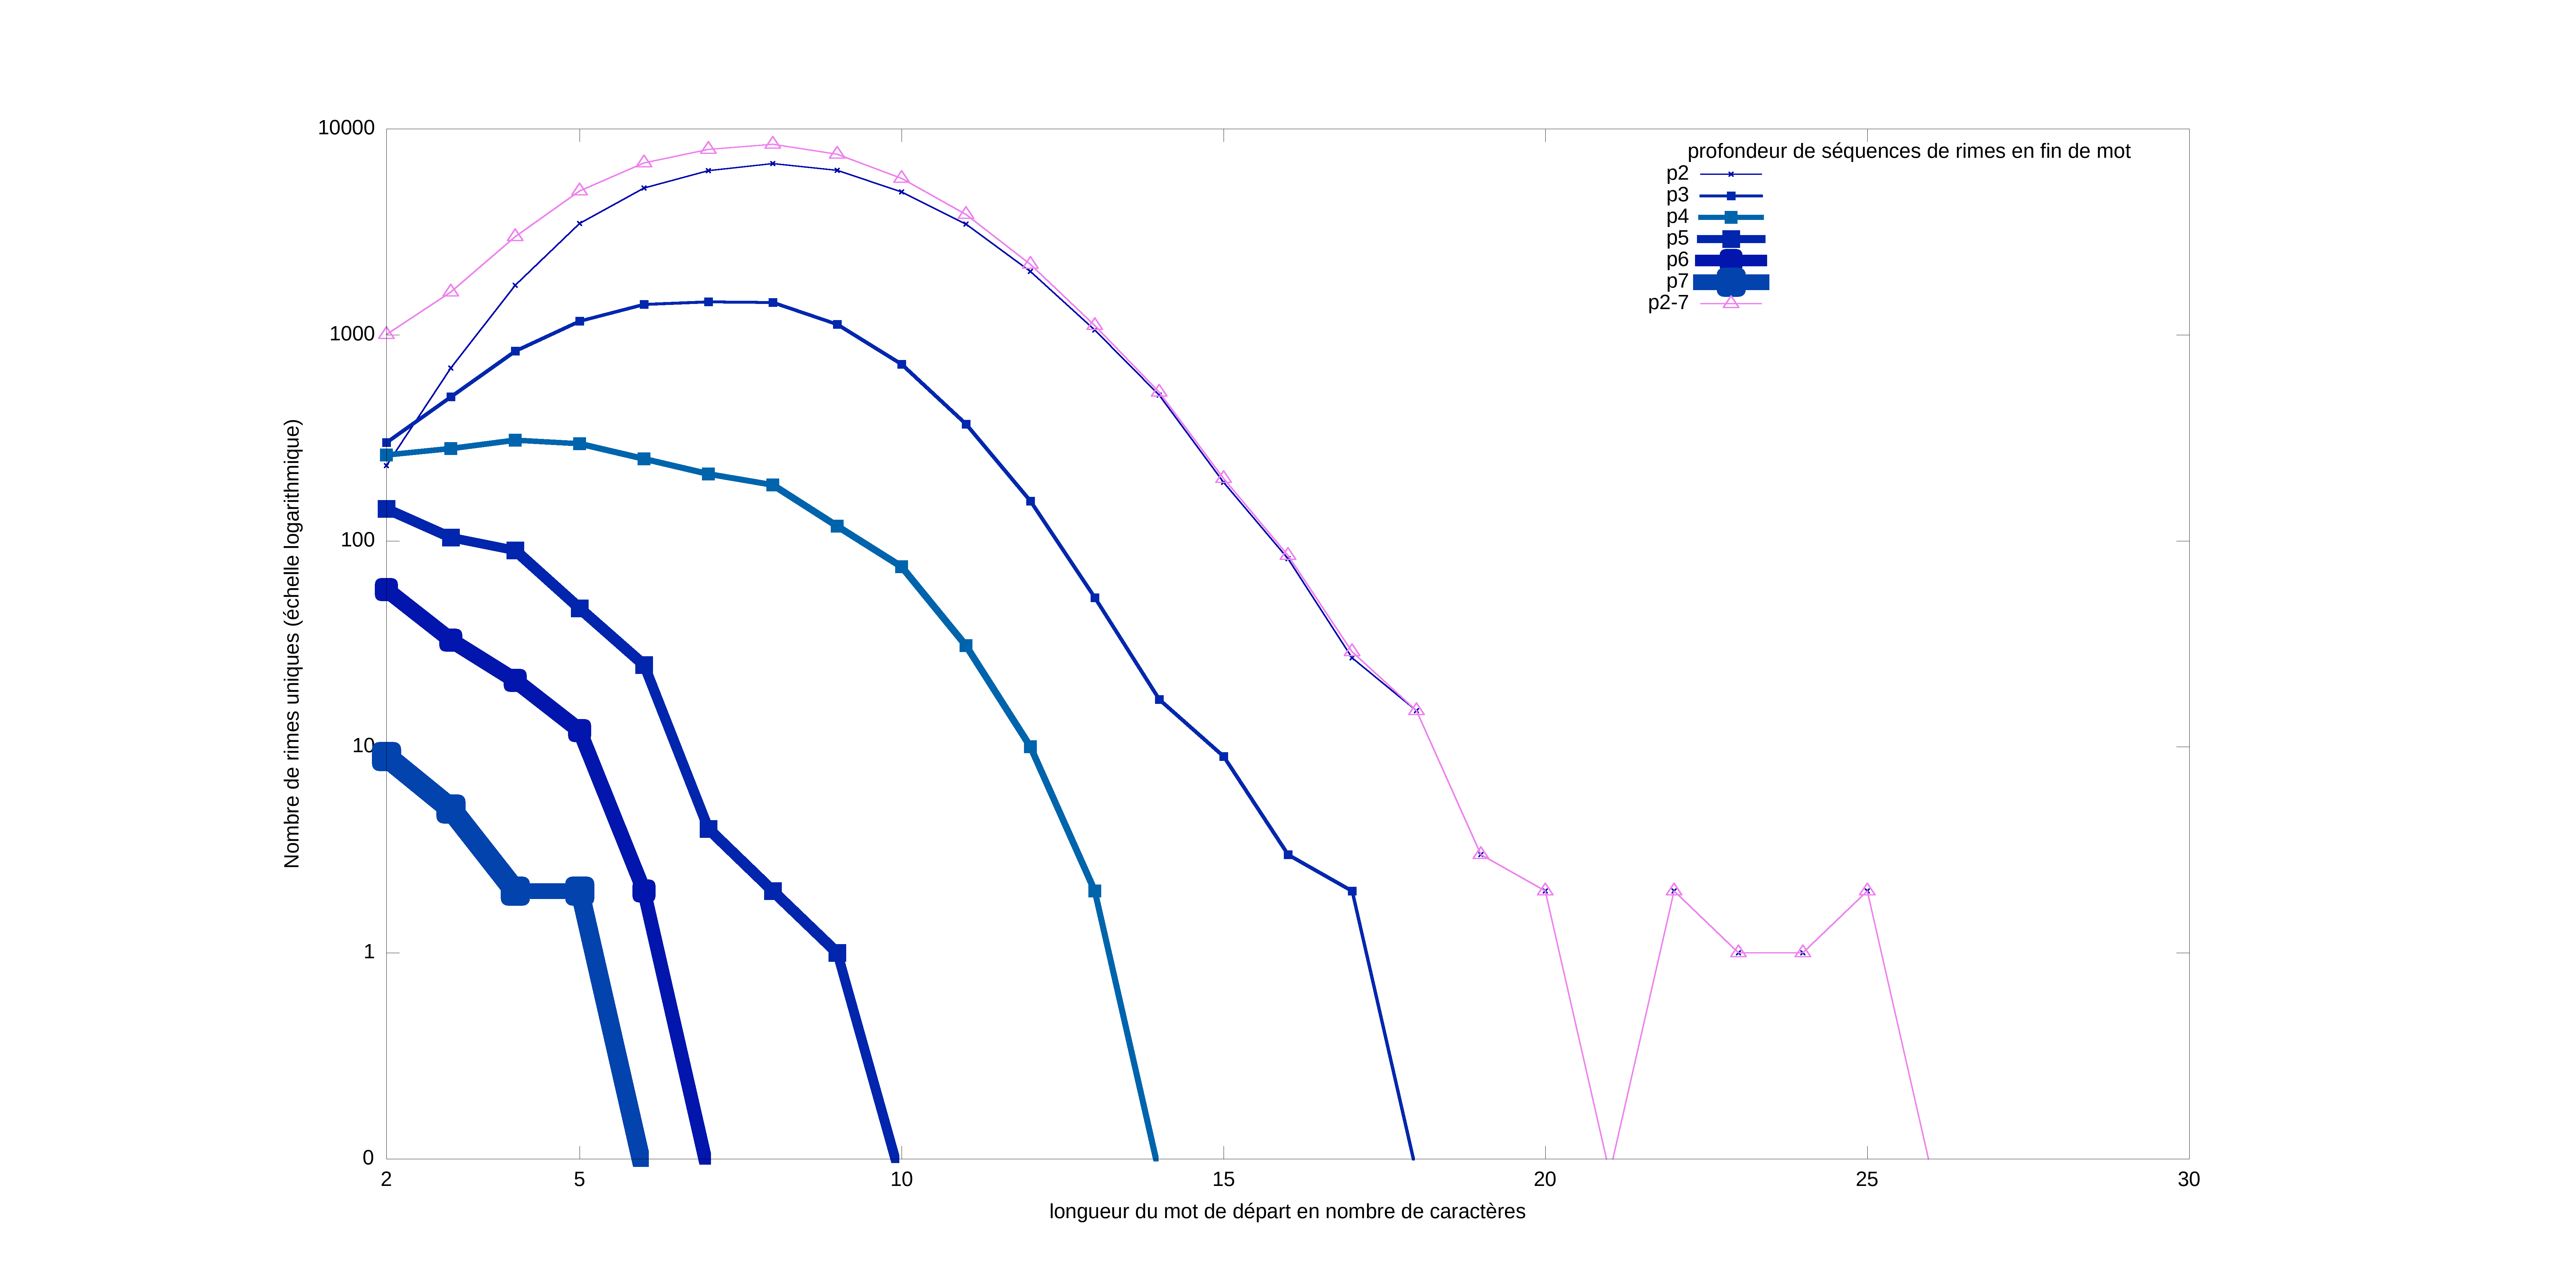
\includegraphics[width=\textwidth]{/home/olivier/Encfs/Privé/ENCRYPTED/Langages/developpement/poetry_analyze/french/gnuplot/1.png}\\
\underline{Exemples}\\
\paragraph{rimes de 2 lettres dans une profondeur de 2 mots (c'est la courbe p2):\\}
\texttt{\colorbox{yellow}{\textbf{oc}};r\colorbox{yellow}{\textbf{oc}} | \colorbox{yellow}{\textbf{pi}};é\colorbox{yellow}{\textbf{pi}} | \colorbox{yellow}{\textbf{in}};l\colorbox{yellow}{\textbf{in}} | \colorbox{yellow}{\textbf{un}};H\colorbox{yellow}{\textbf{un}} | \colorbox{yellow}{\textbf{ut}};b\colorbox{yellow}{\textbf{ut}} | \colorbox{yellow}{\textbf{ru}};b\colorbox{yellow}{\textbf{ru}} | \colorbox{yellow}{\textbf{ru}};c\colorbox{yellow}{\textbf{ru}} |} etc.\\
\\
\paragraph{rimes de 2 lettres dans une profondeur de 3 mots (c'est la courbe p3):\\}
\texttt{\colorbox{yellow}{\textbf{as}};m\colorbox{yellow}{\textbf{as}};am\colorbox{yellow}{\textbf{as}} | \colorbox{yellow}{\textbf{oc}};r\colorbox{yellow}{\textbf{oc}};br\colorbox{yellow}{\textbf{oc}} | \colorbox{yellow}{\textbf{in}};l\colorbox{yellow}{\textbf{in}};cl\colorbox{yellow}{\textbf{in}} | \colorbox{yellow}{\textbf{au}};e\colorbox{yellow}{\textbf{au}};se\colorbox{yellow}{\textbf{au}} |} etc.\\
\\
\paragraph{rimes de 2 lettres dans une profondeur de 7 mots (c'est la courbe p7):\\}
A noter qu'il y en a exactement seulement 9, dont 1 seule qui ne soit pas de la conjugaison de verbes. Je la cite :\\
\texttt{\colorbox{yellow}{\textbf{es}};l\colorbox{yellow}{\textbf{es}};al\colorbox{yellow}{\textbf{es}};tal\colorbox{yellow}{\textbf{es}};étal\colorbox{yellow}{\textbf{es}};pétal\colorbox{yellow}{\textbf{es}};apétal\colorbox{yellow}{\textbf{es}}}\\
\newpage
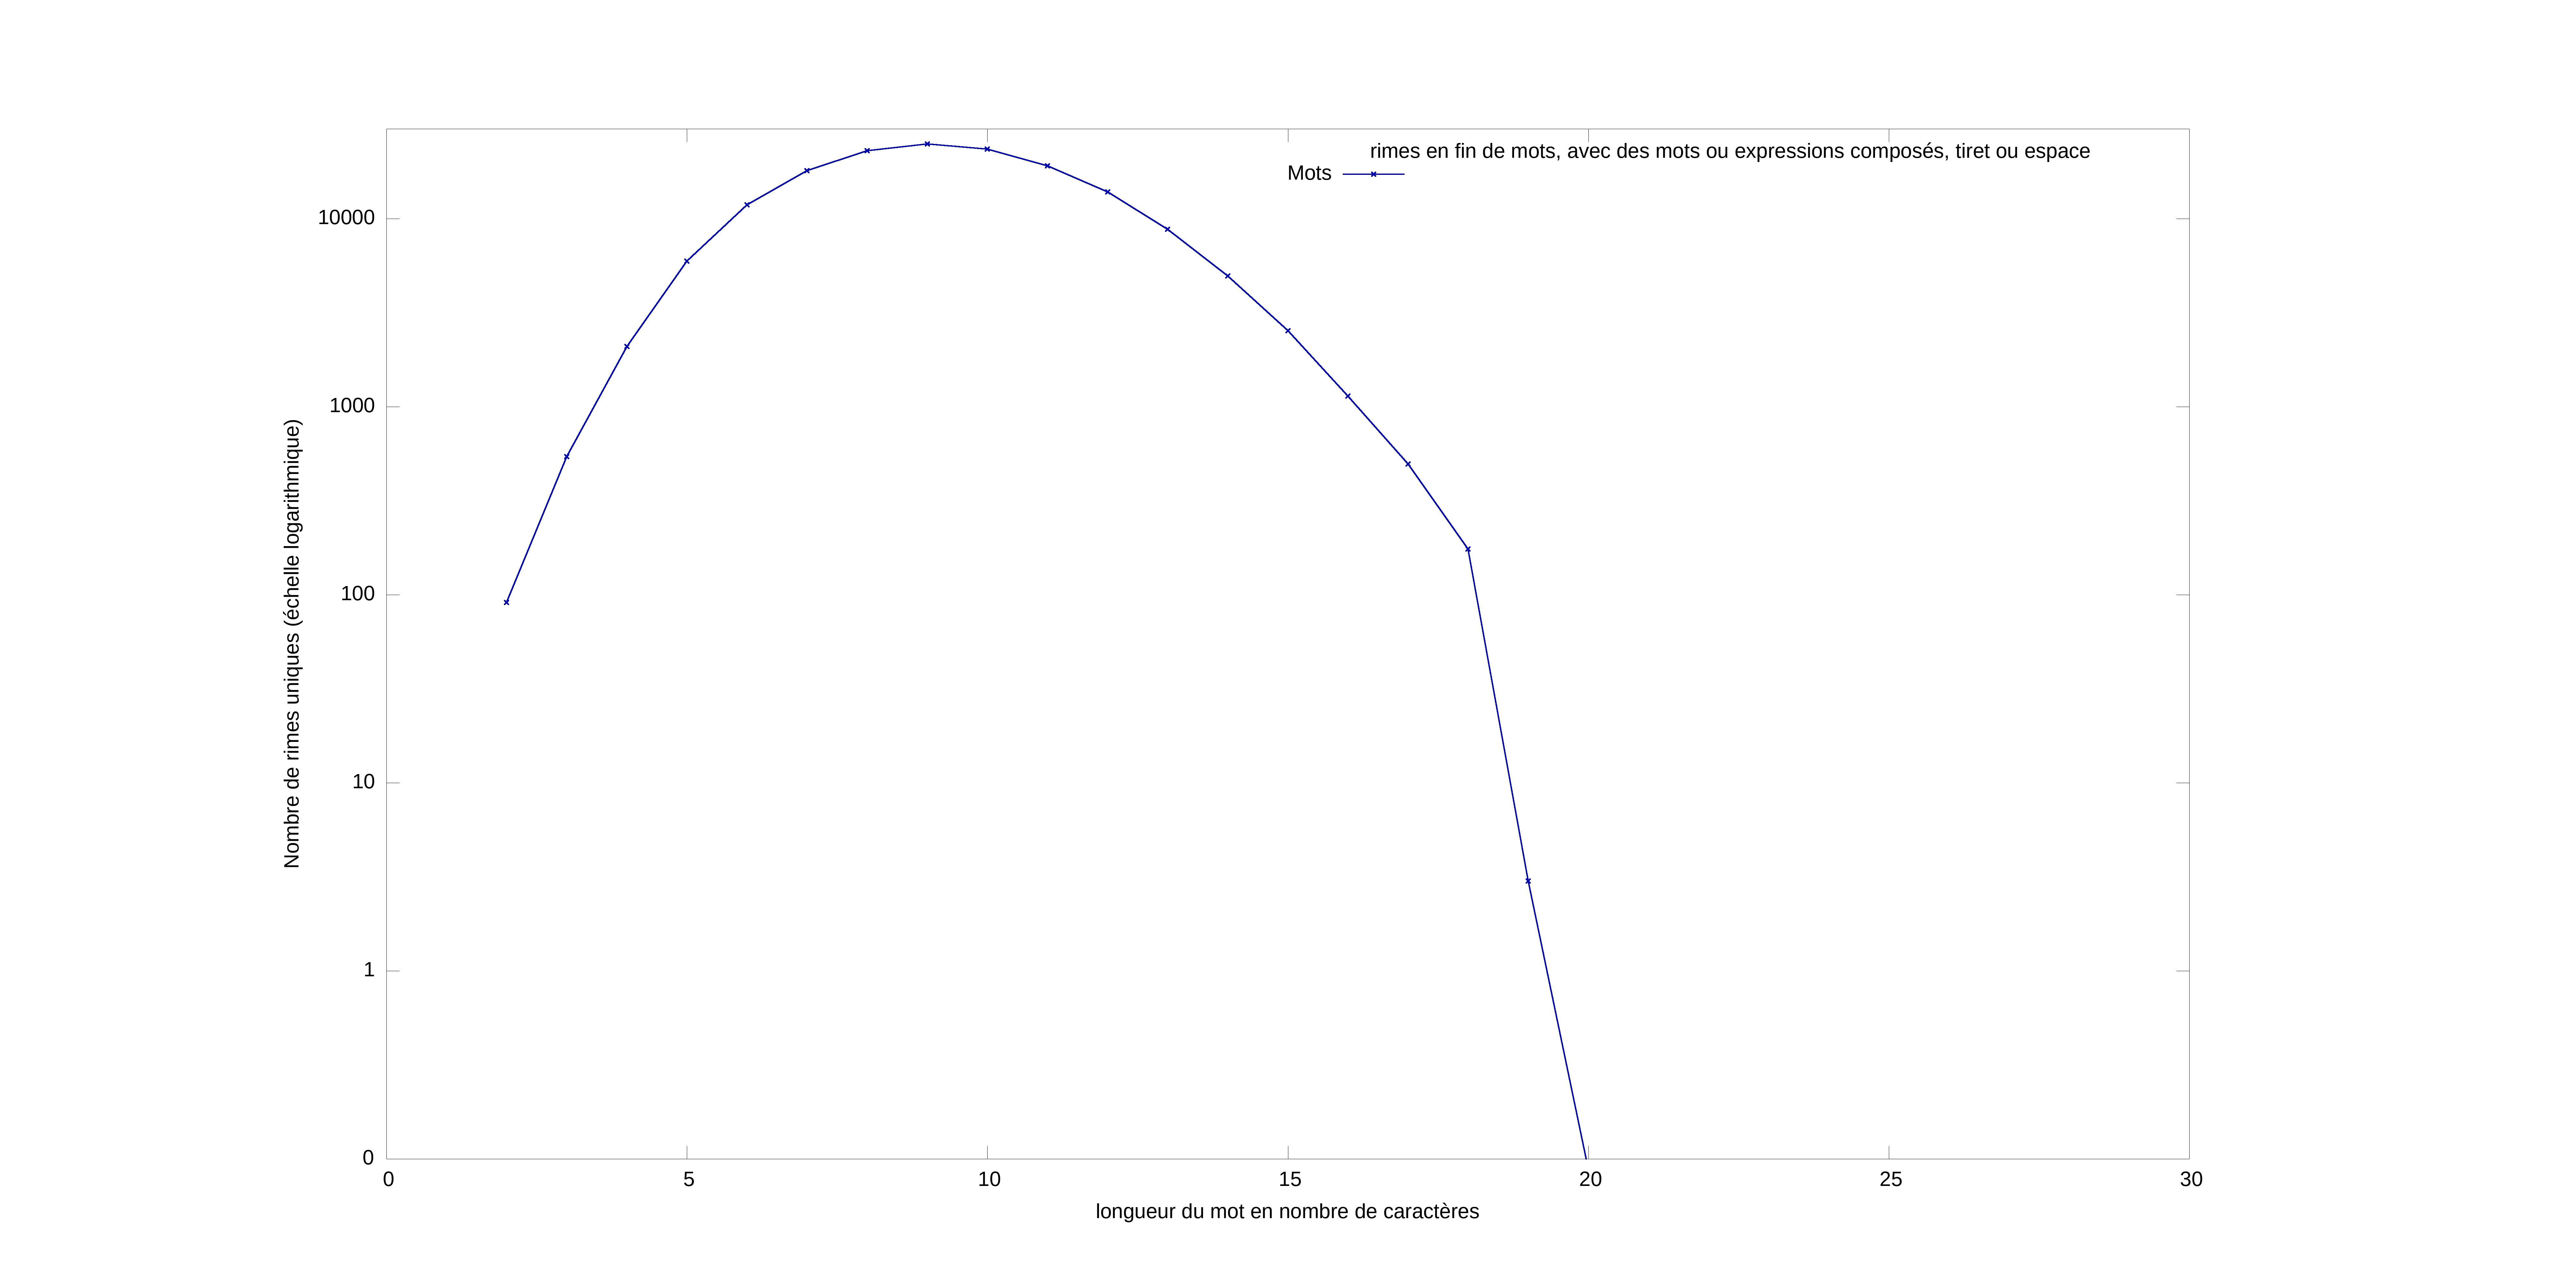
\includegraphics[width=\textwidth]{/home/olivier/Encfs/Privé/ENCRYPTED/Langages/developpement/poetry_analyze/french/gnuplot/4.png}\\
\underline{Exemples}\\
\paragraph{rimes de 2 lettres en fin de mots du dictionnaire, avec des mots ou expression composées (tiret ou espace):\\}
\texttt{cabilla\colorbox{yellow}{\textbf{ud}};entre-nœ\colorbox{yellow}{\textbf{ud}};attrape-niga\colorbox{yellow}{\textbf{ud}}}\\
\textit{oui alors certains se demanderont si "ud" est bien un mot de la langue française, et oui c'est bien le cas, il s'agit d'un instrument à cordes pincées !}\\
\paragraph{rimes de 3 lettres en fin de mots du dictionnaire, avec des mots ou expression composées (tiret ou espace):\\}
\texttt{\colorbox{yellow}{\textbf{roc}};b\colorbox{yellow}{\textbf{roc}};c\colorbox{yellow}{\textbf{roc}};f\colorbox{yellow}{\textbf{roc}};t\colorbox{yellow}{\textbf{roc}};péb\colorbox{yellow}{\textbf{roc}};acc\colorbox{yellow}{\textbf{roc}};esc\colorbox{yellow}{\textbf{roc}};racc\colorbox{yellow}{\textbf{roc}}}\\
\paragraph{rimes de 7 lettres en fin de mots du dictionnaire, avec des mots ou expression composées (tiret ou espace):\\}
\texttt{\colorbox{yellow}{\textbf{voyance}};pré\colorbox{yellow}{\textbf{voyance}};mal\colorbox{yellow}{\textbf{voyance}};impré\colorbox{yellow}{\textbf{voyance}};clair\colorbox{yellow}{\textbf{voyance}}}\\
\newpage
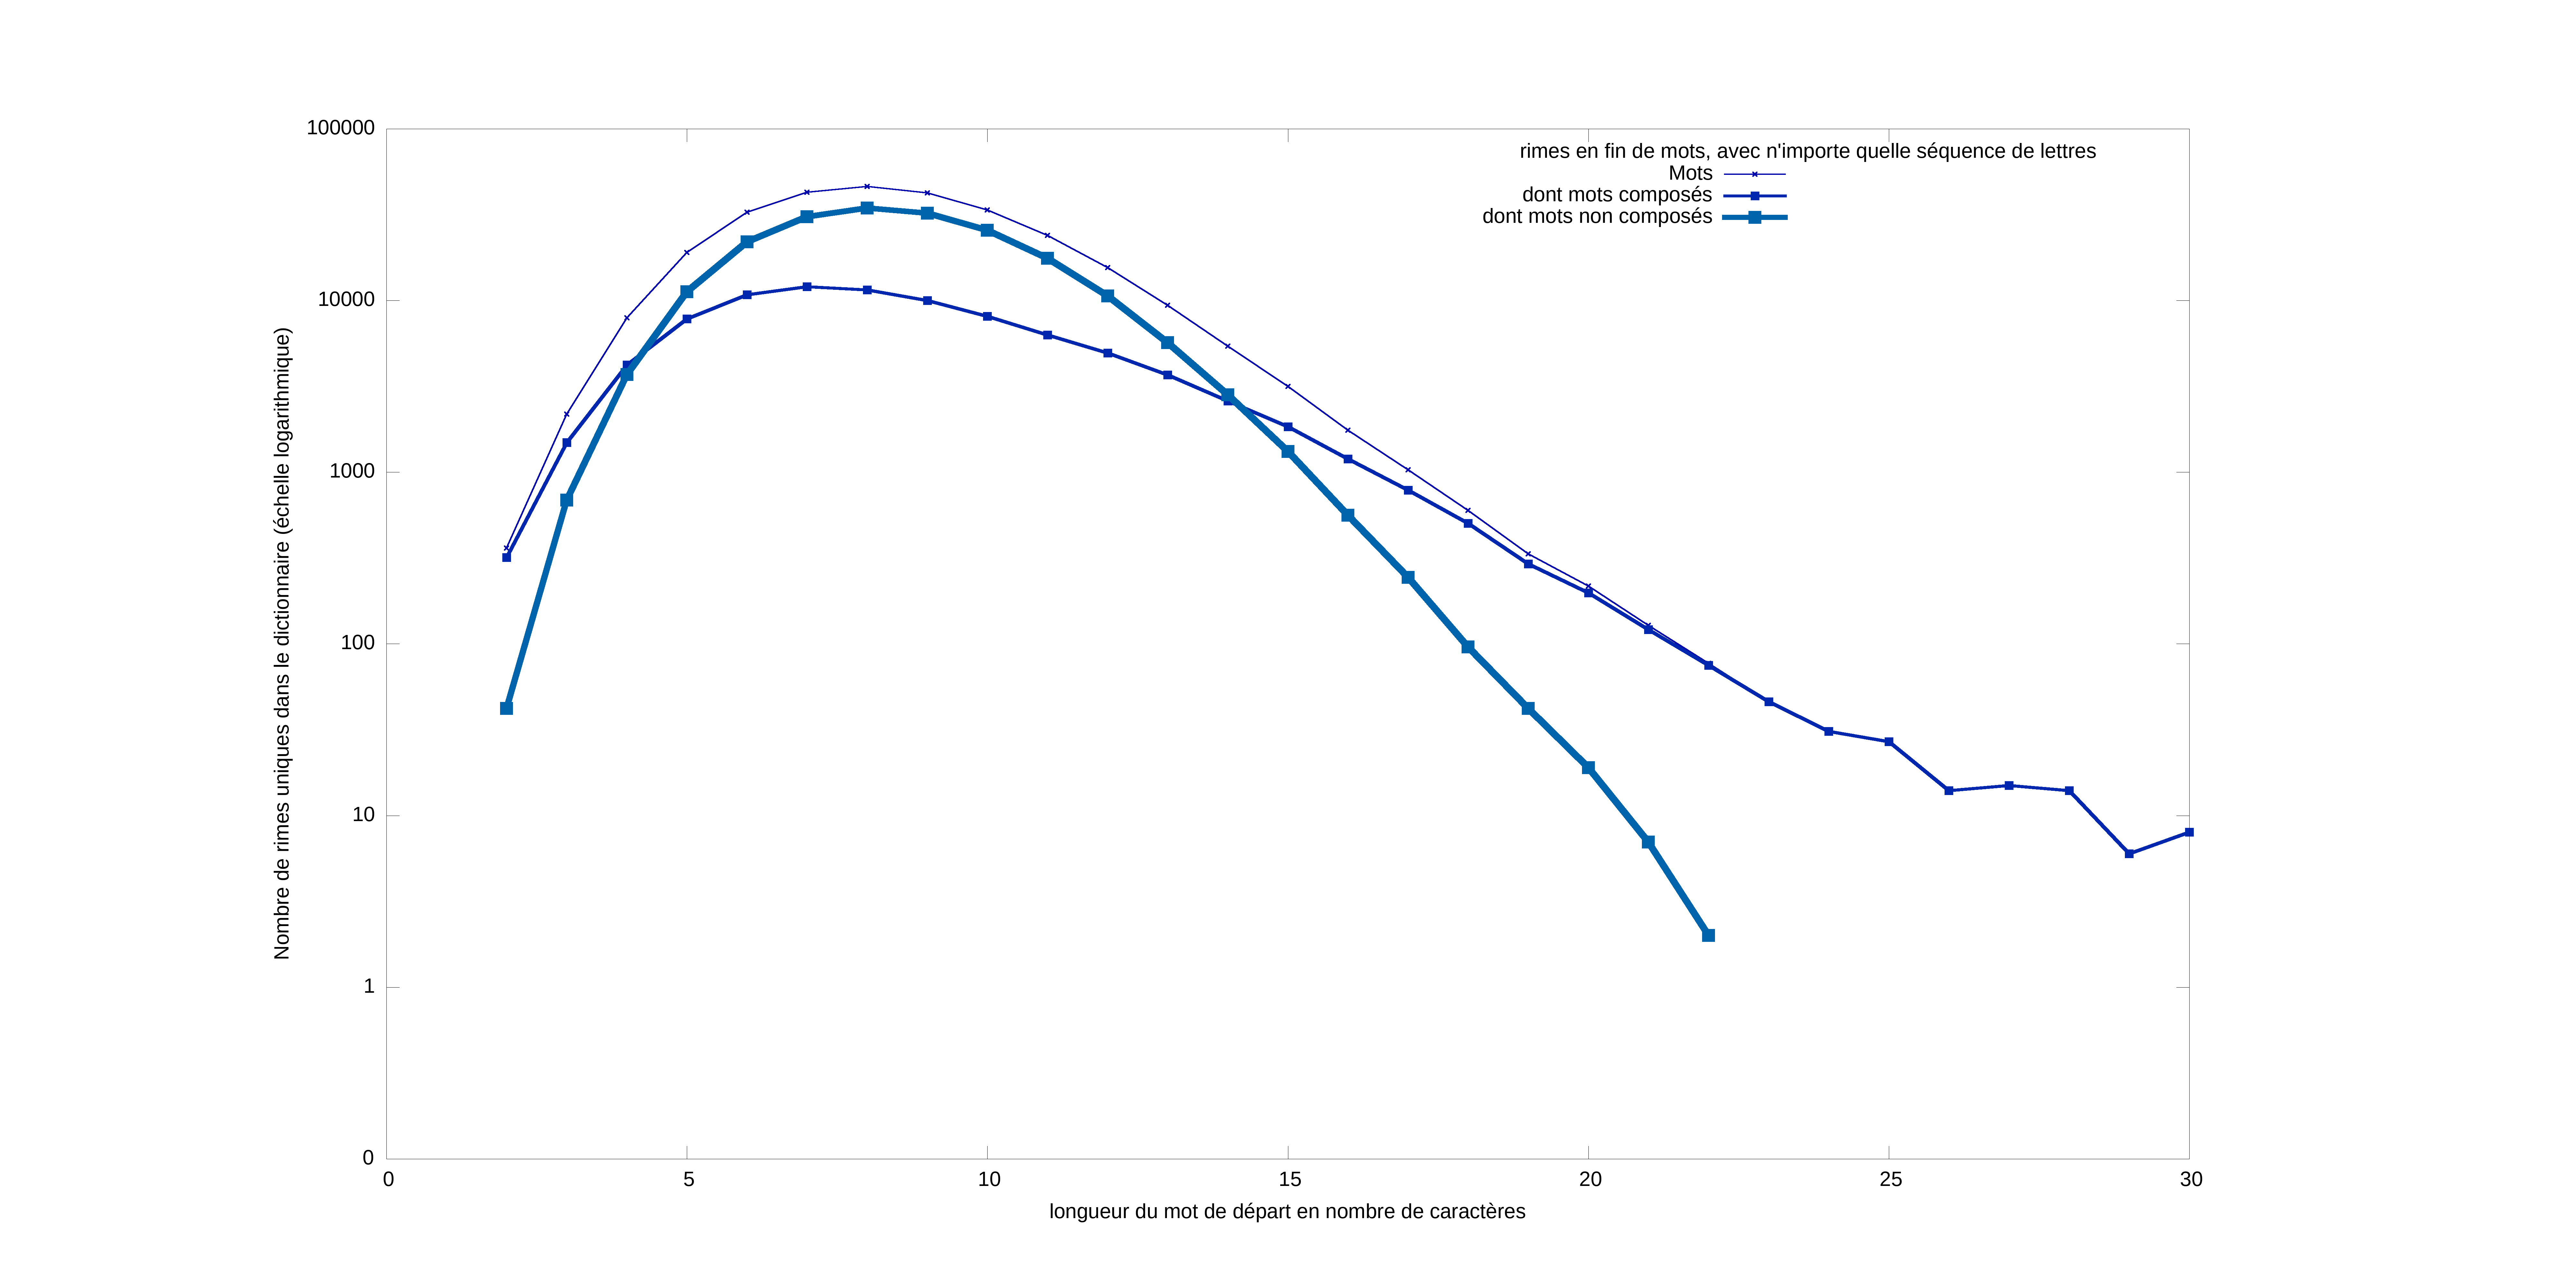
\includegraphics[width=\textwidth]{/home/olivier/Encfs/Privé/ENCRYPTED/Langages/developpement/poetry_analyze/french/gnuplot/5.png}\\
\underline{Exemples}\\
\paragraph{rimes de 2 lettres en fin de mots du dictionnaire, avec n'importe quelle séquence de lettres :\\}
\texttt{mathe\colorbox{yellow}{\textbf{ux}};mafie\colorbox{yellow}{\textbf{ux}};bigle\colorbox{yellow}{\textbf{ux}}}\\
\paragraph{rimes de 7 lettres en fin de mots du dictionnaire, avec n'importe quelle séquence de lettres :\\}
\texttt{\colorbox{yellow}{\textbf{lignage}};dé\colorbox{yellow}{\textbf{lignage}};contre-\colorbox{yellow}{\textbf{lignage}};inter\colorbox{yellow}{\textbf{lignage}};sur\colorbox{yellow}{\textbf{lignage}};sou\colorbox{yellow}{\textbf{lignage}}}\\
\paragraph{rimes de 14 lettres en fin de mots du dictionnaire, avec n'importe quelle séquence de lettres :\\}
\texttt{\colorbox{yellow}{\textbf{sensibilisation}};dé\colorbox{yellow}{\textbf{sensibilisation}};in\colorbox{yellow}{\textbf{sensibilisation}};photo\colorbox{yellow}{\textbf{sensibilisation}};hyper\colorbox{yellow}{\textbf{sensibilisation}}}\\
\newpage
\subsection{Rimes à l'oeil en début de mots}
\subsubsection{profondeur de rimes}
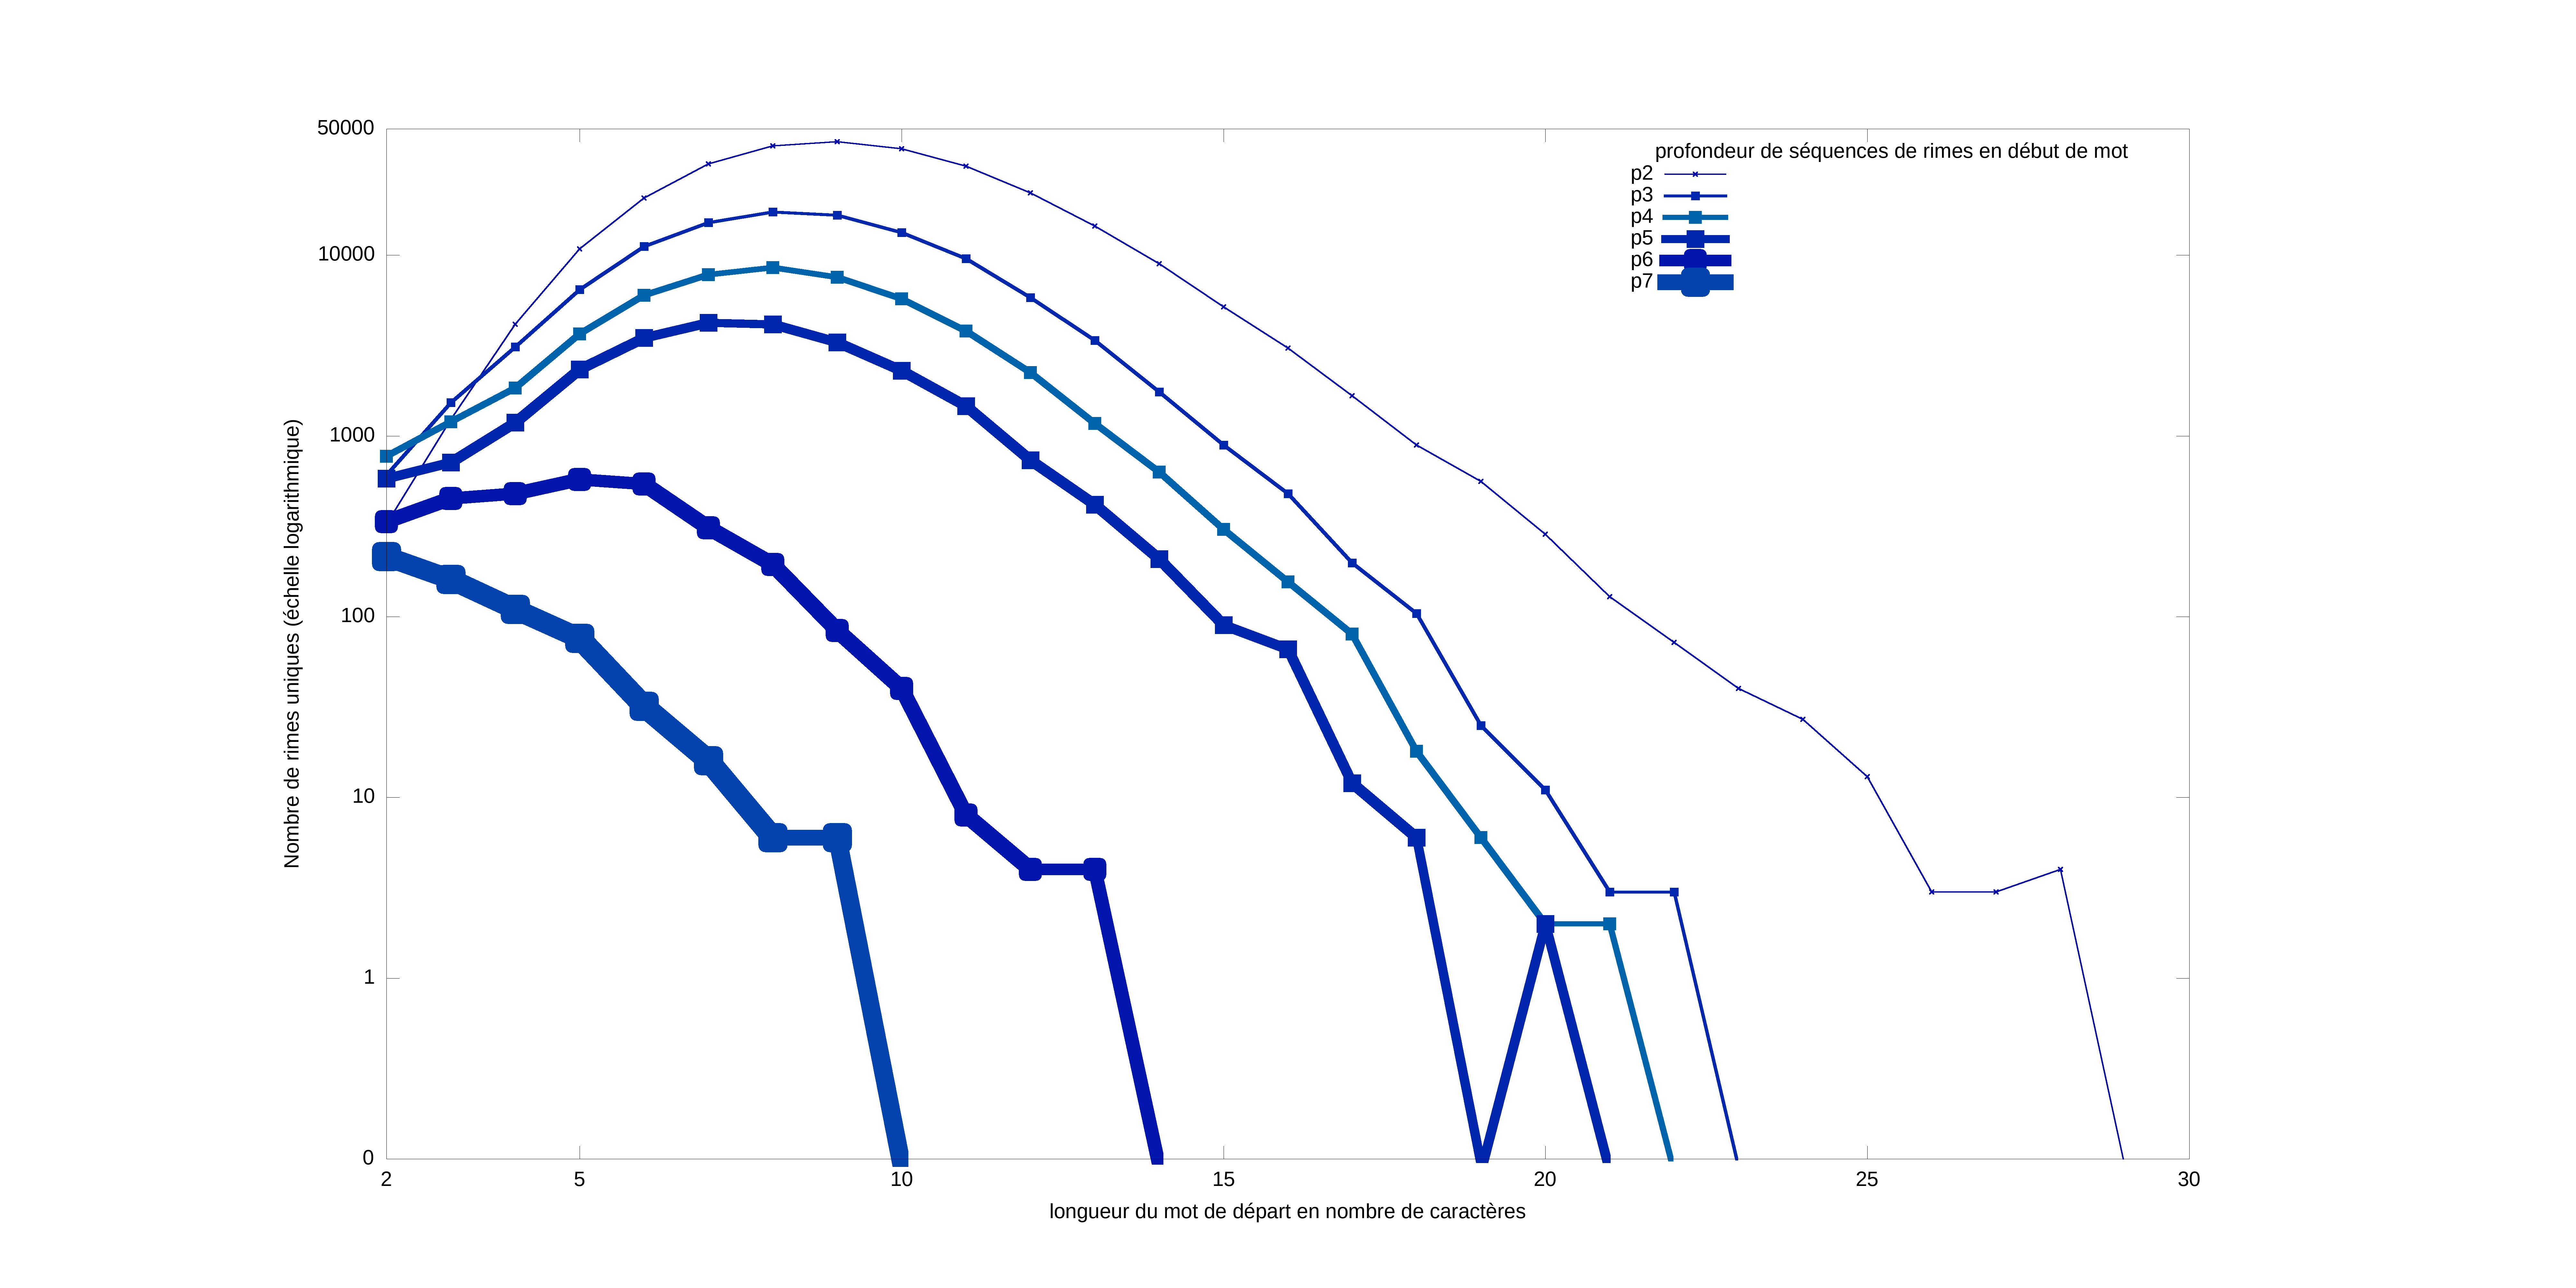
\includegraphics[width=\textwidth]{/home/olivier/Encfs/Privé/ENCRYPTED/Langages/developpement/poetry_analyze/french/gnuplot/2.png}\\
\underline{Exemples}\\
\paragraph{rimes de 3 lettres en début de mots du dictionnaire, profondeur de 3 mots :\\}
\texttt{\colorbox{yellow}{\textbf{lux}};\colorbox{yellow}{\textbf{lux}}e;\colorbox{yellow}{\textbf{lux}}er}\\
\paragraph{rimes de 3 lettres en début de mots du dictionnaire, profondeur de 4 mots :\\}
\texttt{\colorbox{yellow}{\textbf{tir}};\colorbox{yellow}{\textbf{tir}}e;\colorbox{yellow}{\textbf{tir}}et;\colorbox{yellow}{\textbf{tir}}eté}\\
\paragraph{rimes de 7 lettres en début de mots du dictionnaire, profondeur de 3 mots :\\}
\texttt{\colorbox{yellow}{\textbf{romance}};\colorbox{yellow}{\textbf{romance}}r;\colorbox{yellow}{\textbf{romance}}ro}\\
\newpage
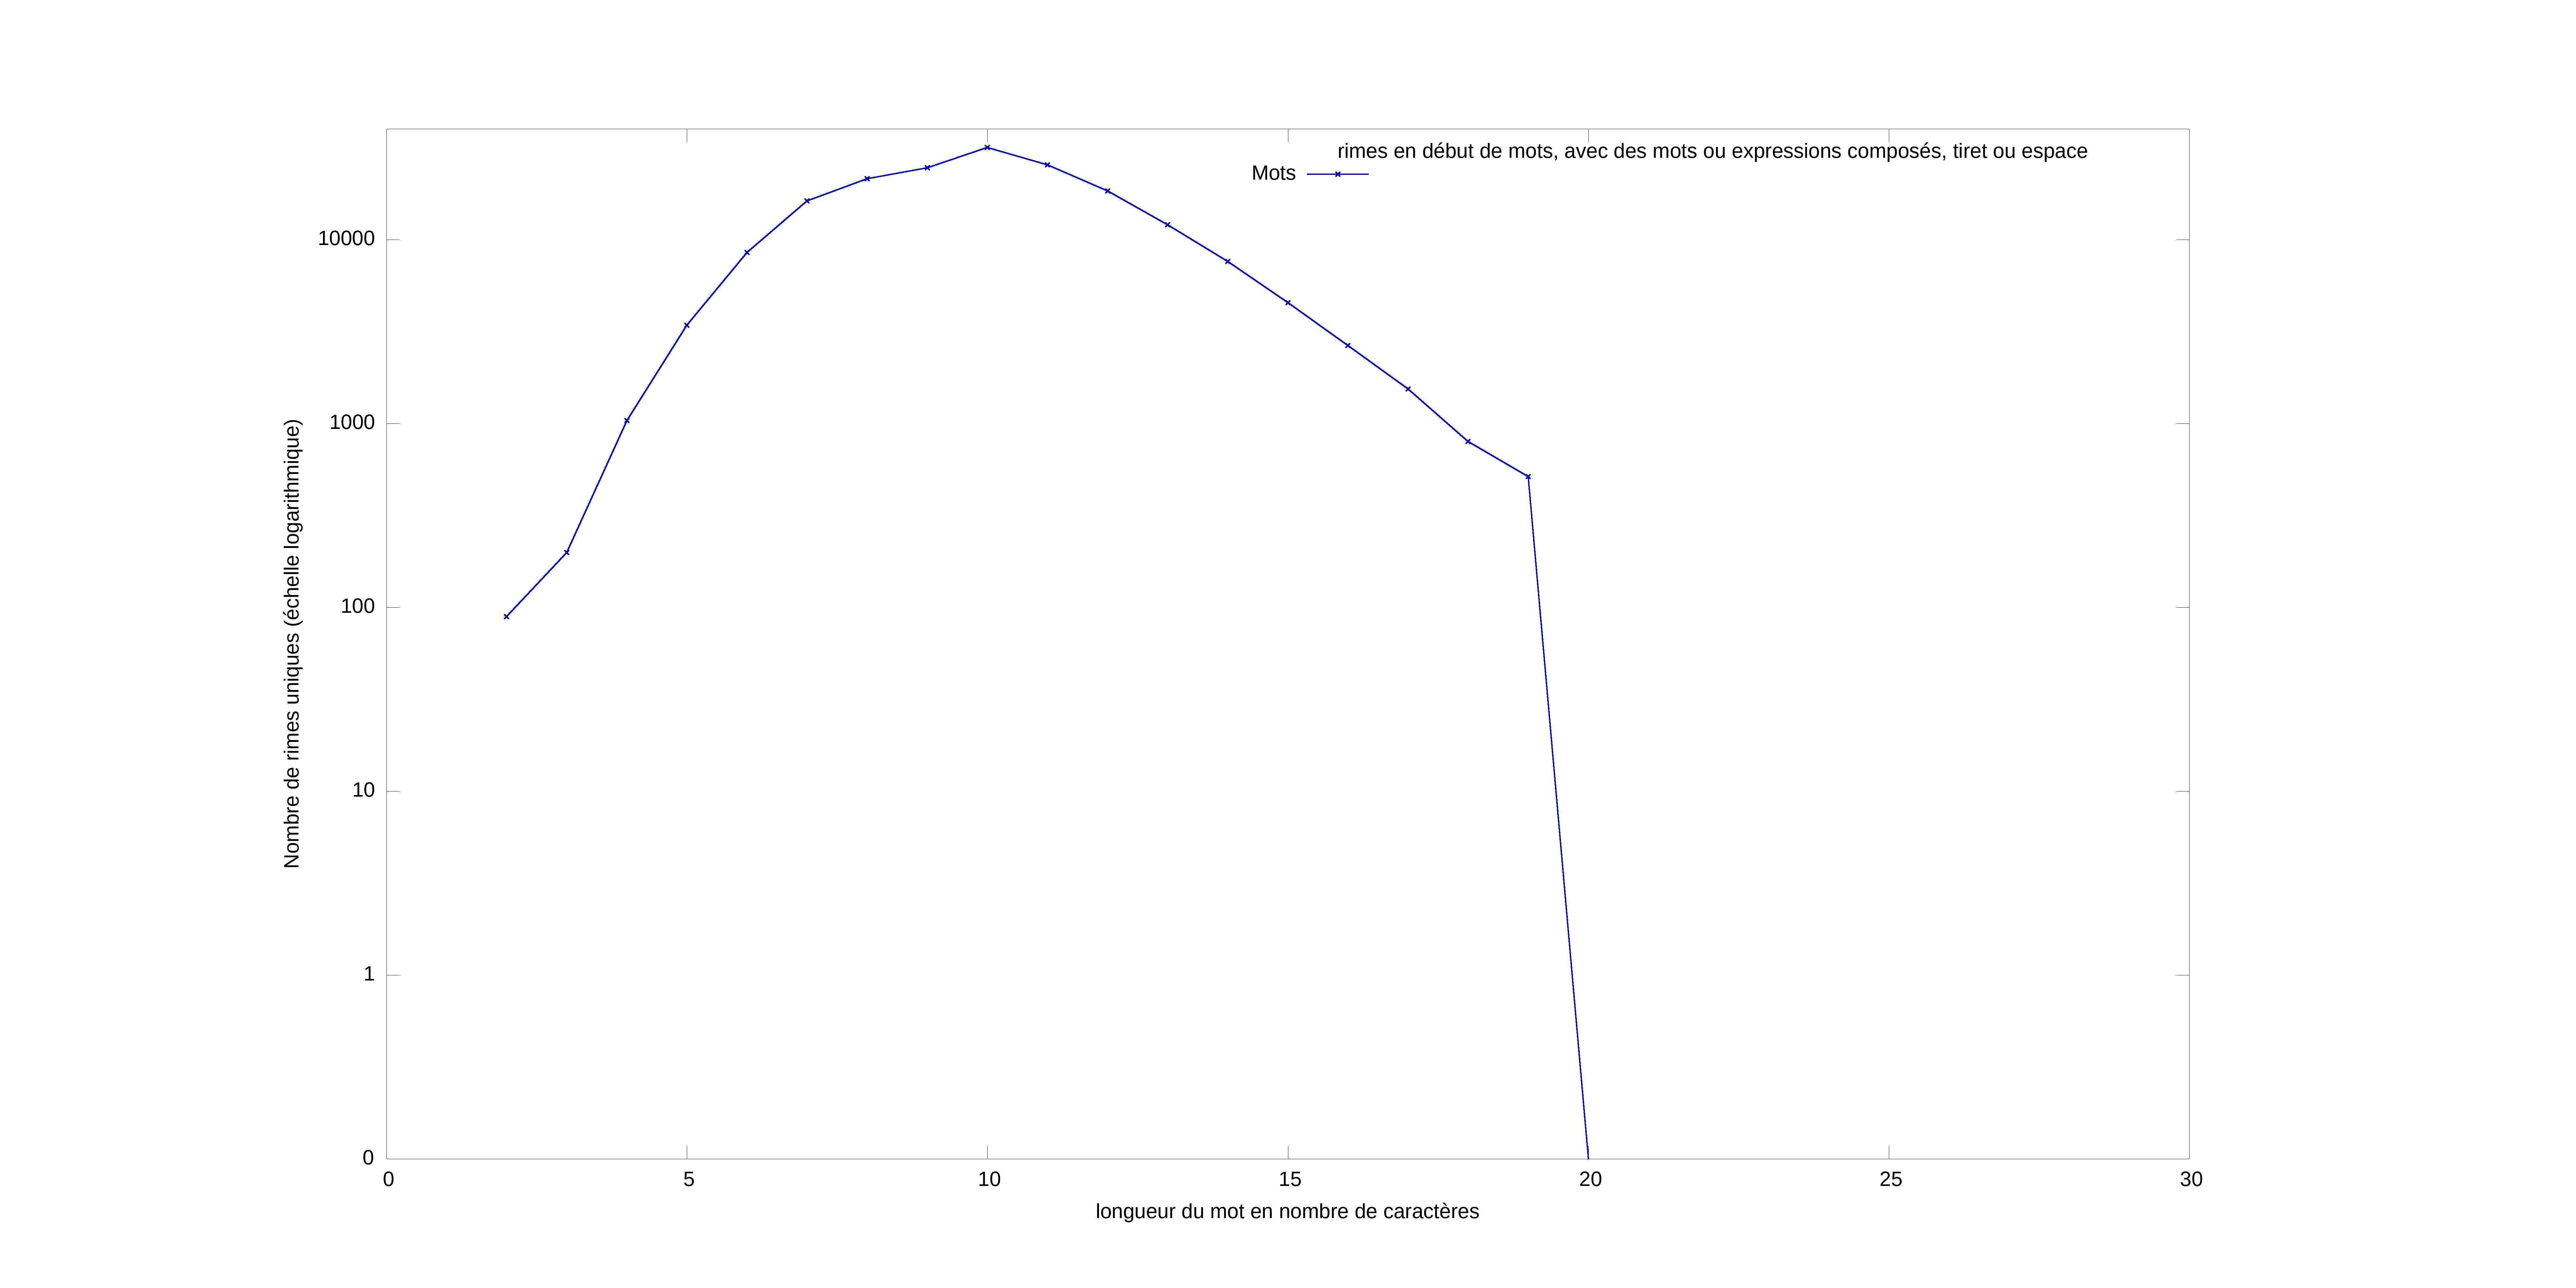
\includegraphics[width=\textwidth]{/home/olivier/Encfs/Privé/ENCRYPTED/Langages/developpement/poetry_analyze/french/gnuplot/3.png}\\
\underline{Exemples}\\
\paragraph{rimes composés d'un mot du dictionnaire, de 5 lettres, en début de mot :\\}
\texttt{\colorbox{yellow}{\textbf{alloc}};\colorbox{yellow}{\textbf{alloc}}ation;\colorbox{yellow}{\textbf{alloc}}htone;\colorbox{yellow}{\textbf{alloc}}ution;\colorbox{yellow}{\textbf{alloc}}ataire;\colorbox{yellow}{\textbf{alloc}}atrice;\colorbox{yellow}{\textbf{alloc}}utaire;}\\
\texttt{\colorbox{yellow}{\textbf{alloc}}entrique;\colorbox{yellow}{\textbf{alloc}}entrisme}\\
\paragraph{rimes composés d'un mot du dictionnaire, de 15 lettres, en début de mot :\\}
\texttt{\colorbox{yellow}{\textbf{incommensurable}};\colorbox{yellow}{\textbf{incommensurable}}ment}\\
\newpage
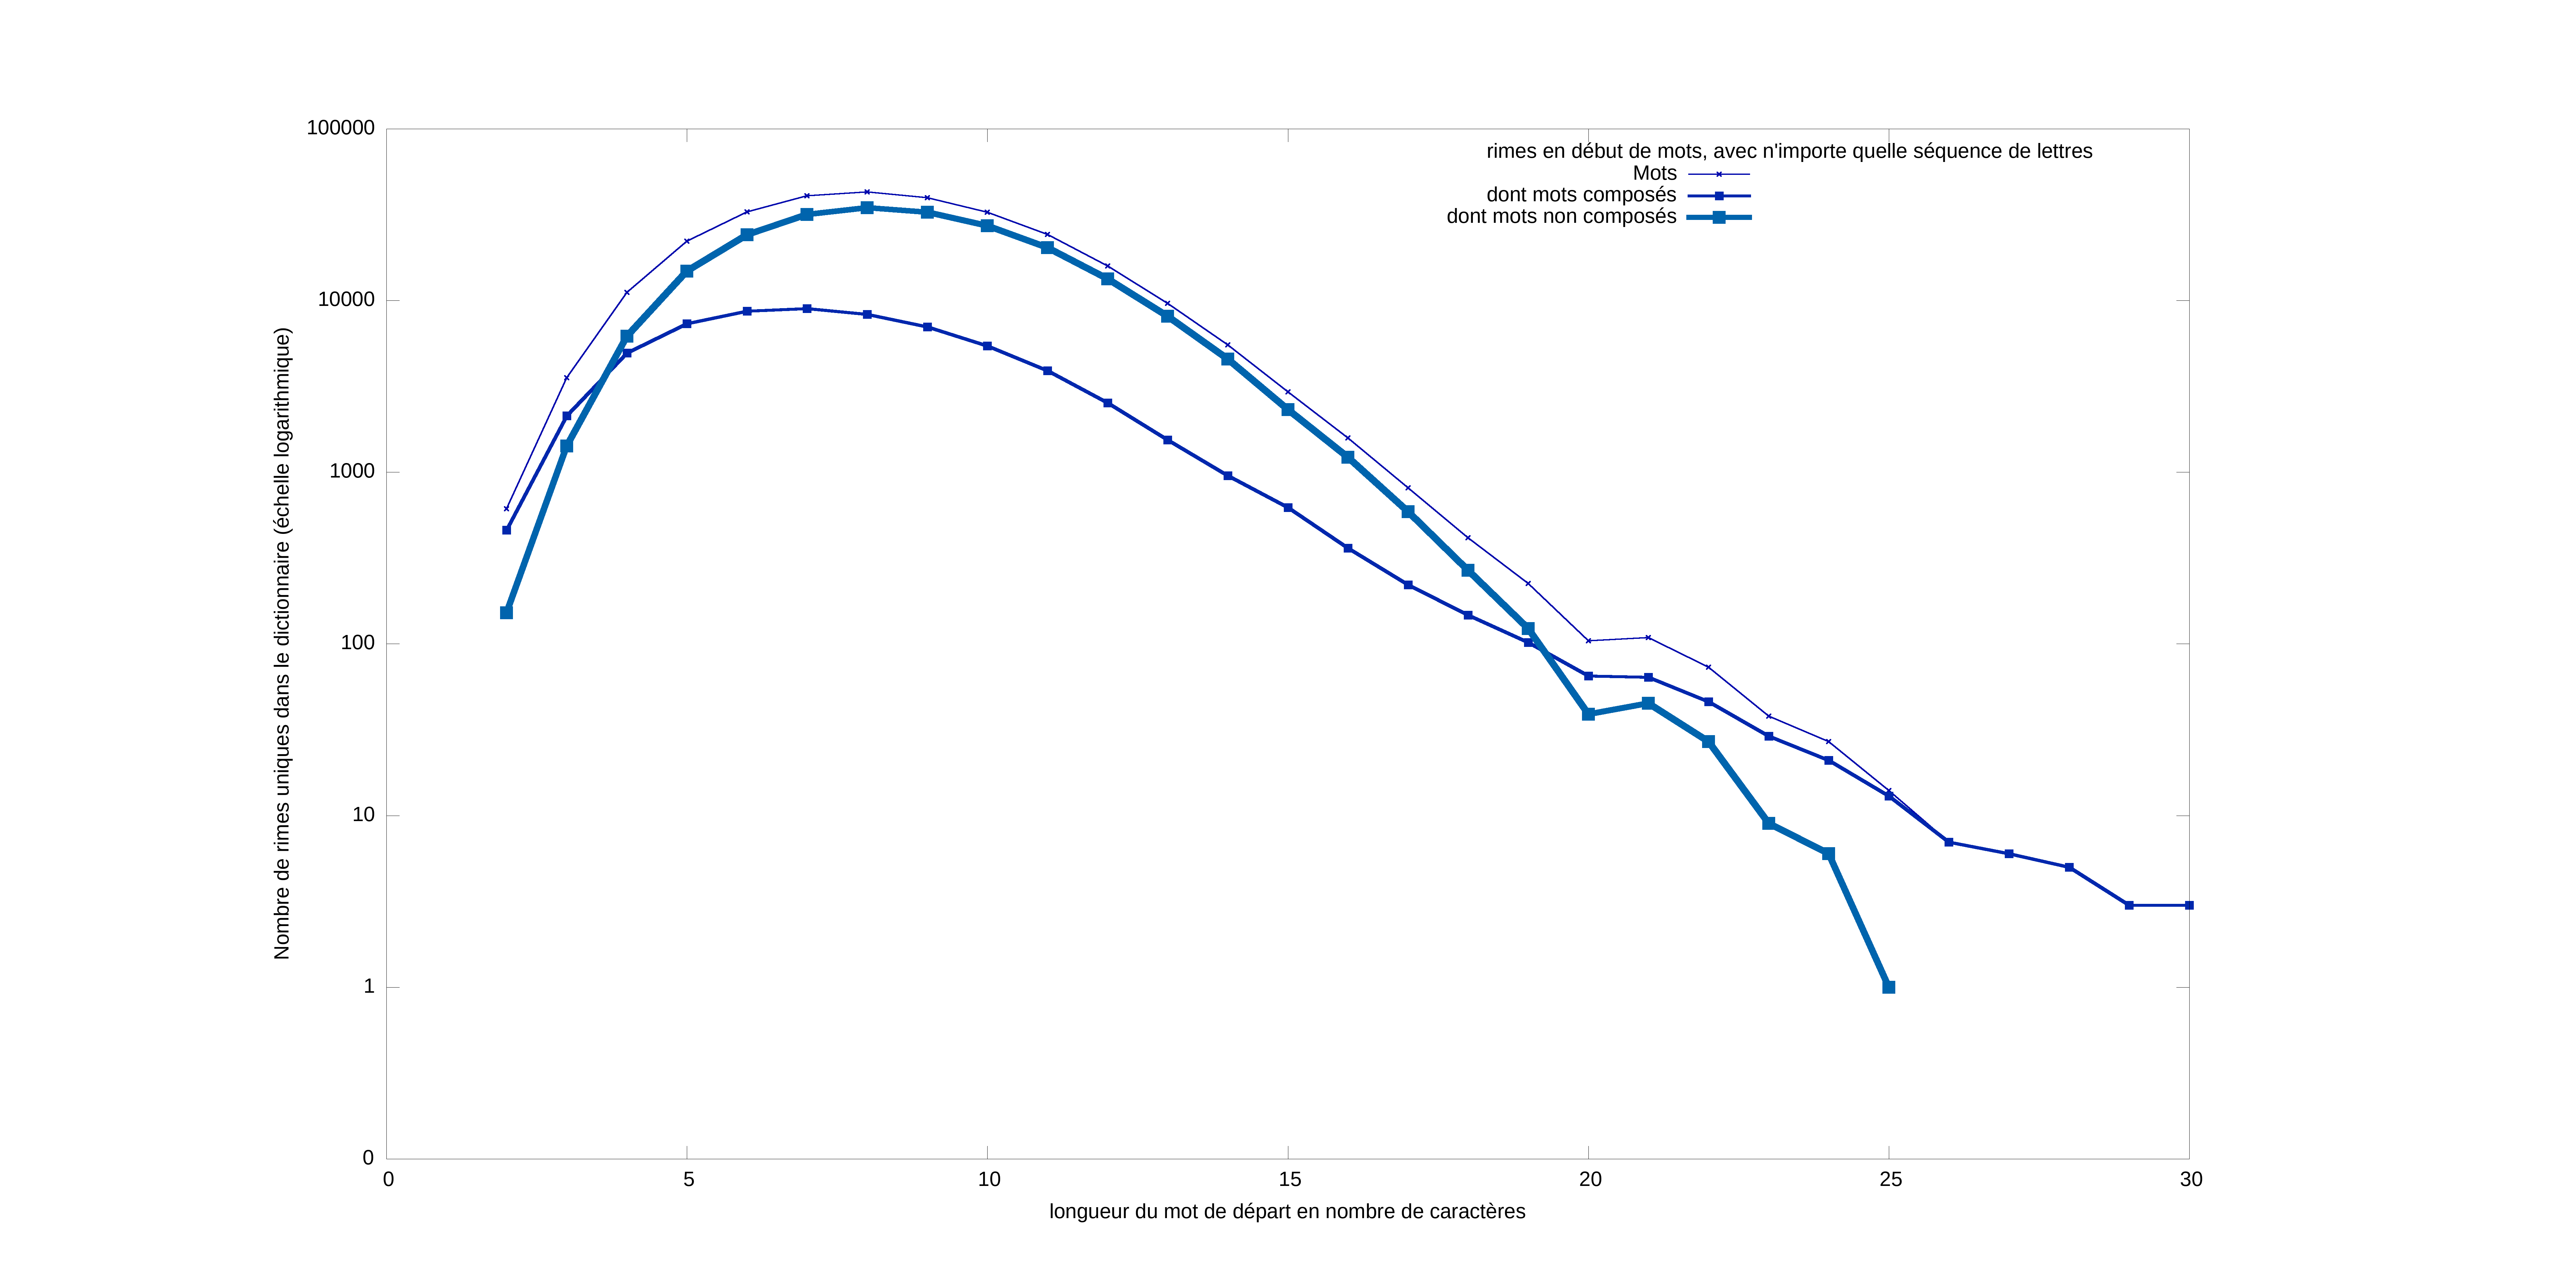
\includegraphics[width=\textwidth]{/home/olivier/Encfs/Privé/ENCRYPTED/Langages/developpement/poetry_analyze/french/gnuplot/6.png}\\
\underline{Exemples}\\
\paragraph{rimes de 8 lettres en début de mot :\\}
\texttt{\colorbox{yellow}{\textbf{accouche}}ment;\colorbox{yellow}{\textbf{accouche}}r;\colorbox{yellow}{\textbf{accouche}}use}\\
\newpage
\subsection{Rimes à l'oeil "glissantes"}
\underline{Voici des exemples de rimes à l'oeil  "glissantes :"}
\paragraph{rimes glissante de 2 lettres sur une profondeur de 9 mots :\\}
\texttt{\colorbox{yellow}{\textbf{at}}axie;b\colorbox{yellow}{\textbf{at}}ave;ab\colorbox{yellow}{\textbf{at}}ée;agn\colorbox{yellow}{\textbf{at}}e;acom\colorbox{yellow}{\textbf{at}}}
\paragraph{rimes glissante de 2 lettres sur une profondeur de 9 mots :\\}
\texttt{\colorbox{yellow}{\textbf{ge}}ignement;a\colorbox{yellow}{\textbf{ge}}ncement;ar\colorbox{yellow}{\textbf{ge}}nterie;con\colorbox{yellow}{\textbf{ge}}lable;abio\colorbox{yellow}{\textbf{ge}}nèse;aména\colorbox{yellow}{\textbf{ge}}use;astrin\colorbox{yellow}{\textbf{ge}}nt;affoura\colorbox{yellow}{\textbf{ge}}r;accrocha\colorbox{yellow}{\textbf{ge}}}
\paragraph{rimes glissante de 9 lettres sur une profondeur de 2 mots :\\}
\texttt{\colorbox{yellow}{\textbf{chronique}}r;a\colorbox{yellow}{\textbf{chronique}}}\\
\\Une fois l'analyse et le classement de toutes les combinaisons possible à partir de l'ensemble des mots communs des dictionnaires récupérés, on obtient le graphique suivant :\\
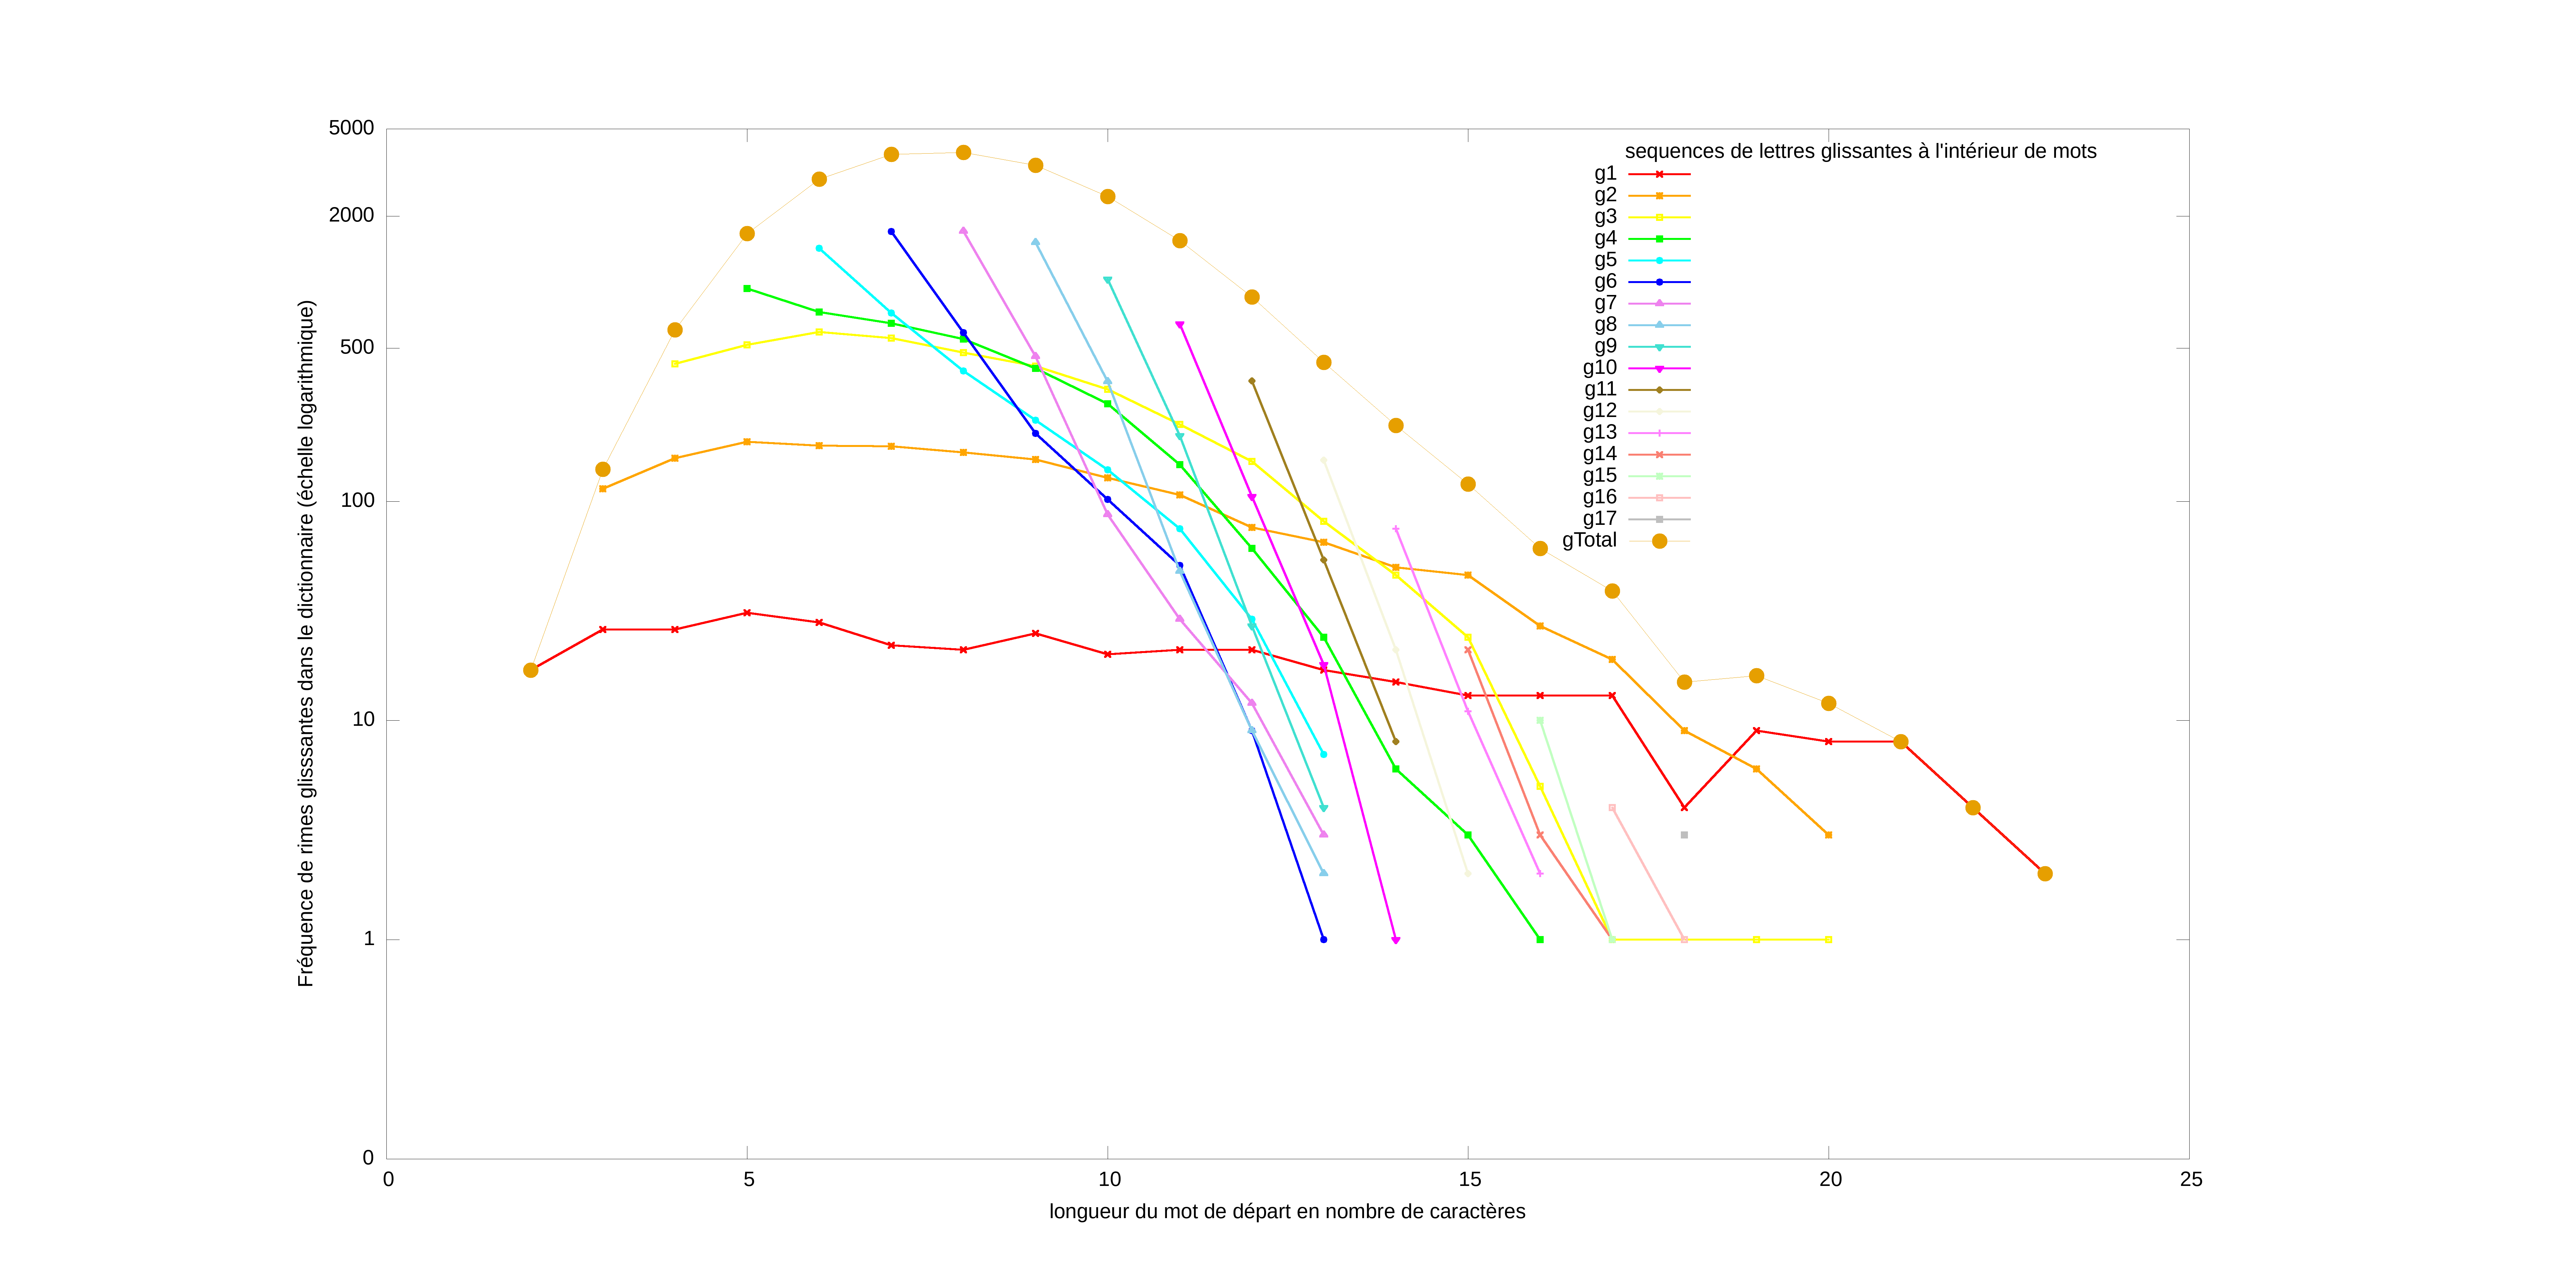
\includegraphics[width=\textwidth]{/home/olivier/Encfs/Privé/ENCRYPTED/Langages/developpement/poetry_analyze/french/gnuplot/7.png}\\
On en déduit que le maximum de rimes glissantes est obtenu pour une longueur de mot de départ de 8 lettres.\\
\\On note également une "extinction" progressive du nombre de rimes glissantes qui suit asymptotiquement une courbe mathématique, dans chaque cas de figure.\\
\\Et surtout, les données cumulées de toutes les combinaisons de rimes glissantes pour une longueur de mot, sont assez remarquables : elles s'approchent d'une courbe limite bien particulière, représentées par gTotal sur le graphique ci-dessus.\\
\\Le positionnement interne des lettres de l'alphabet dans les mots du dictionnaire n'est pas lié au hasard, il y a une ou des contrainte(s) mathématique dans l'élaboration d'un mot, et donc aussi dans les nouveaux mots qui apparaissent ou disparaissent au fur et à mesure du temps dans les dictionnaires de la langue.\\
\\On dirait que les mots sont liés les uns aux autres, par des règles qui nous échappent encore ?\\
\\Et pourquoi n'en n'avons-nous pas conscience naturellement ?\\
\subsection{Rimes sonores en début de mots}
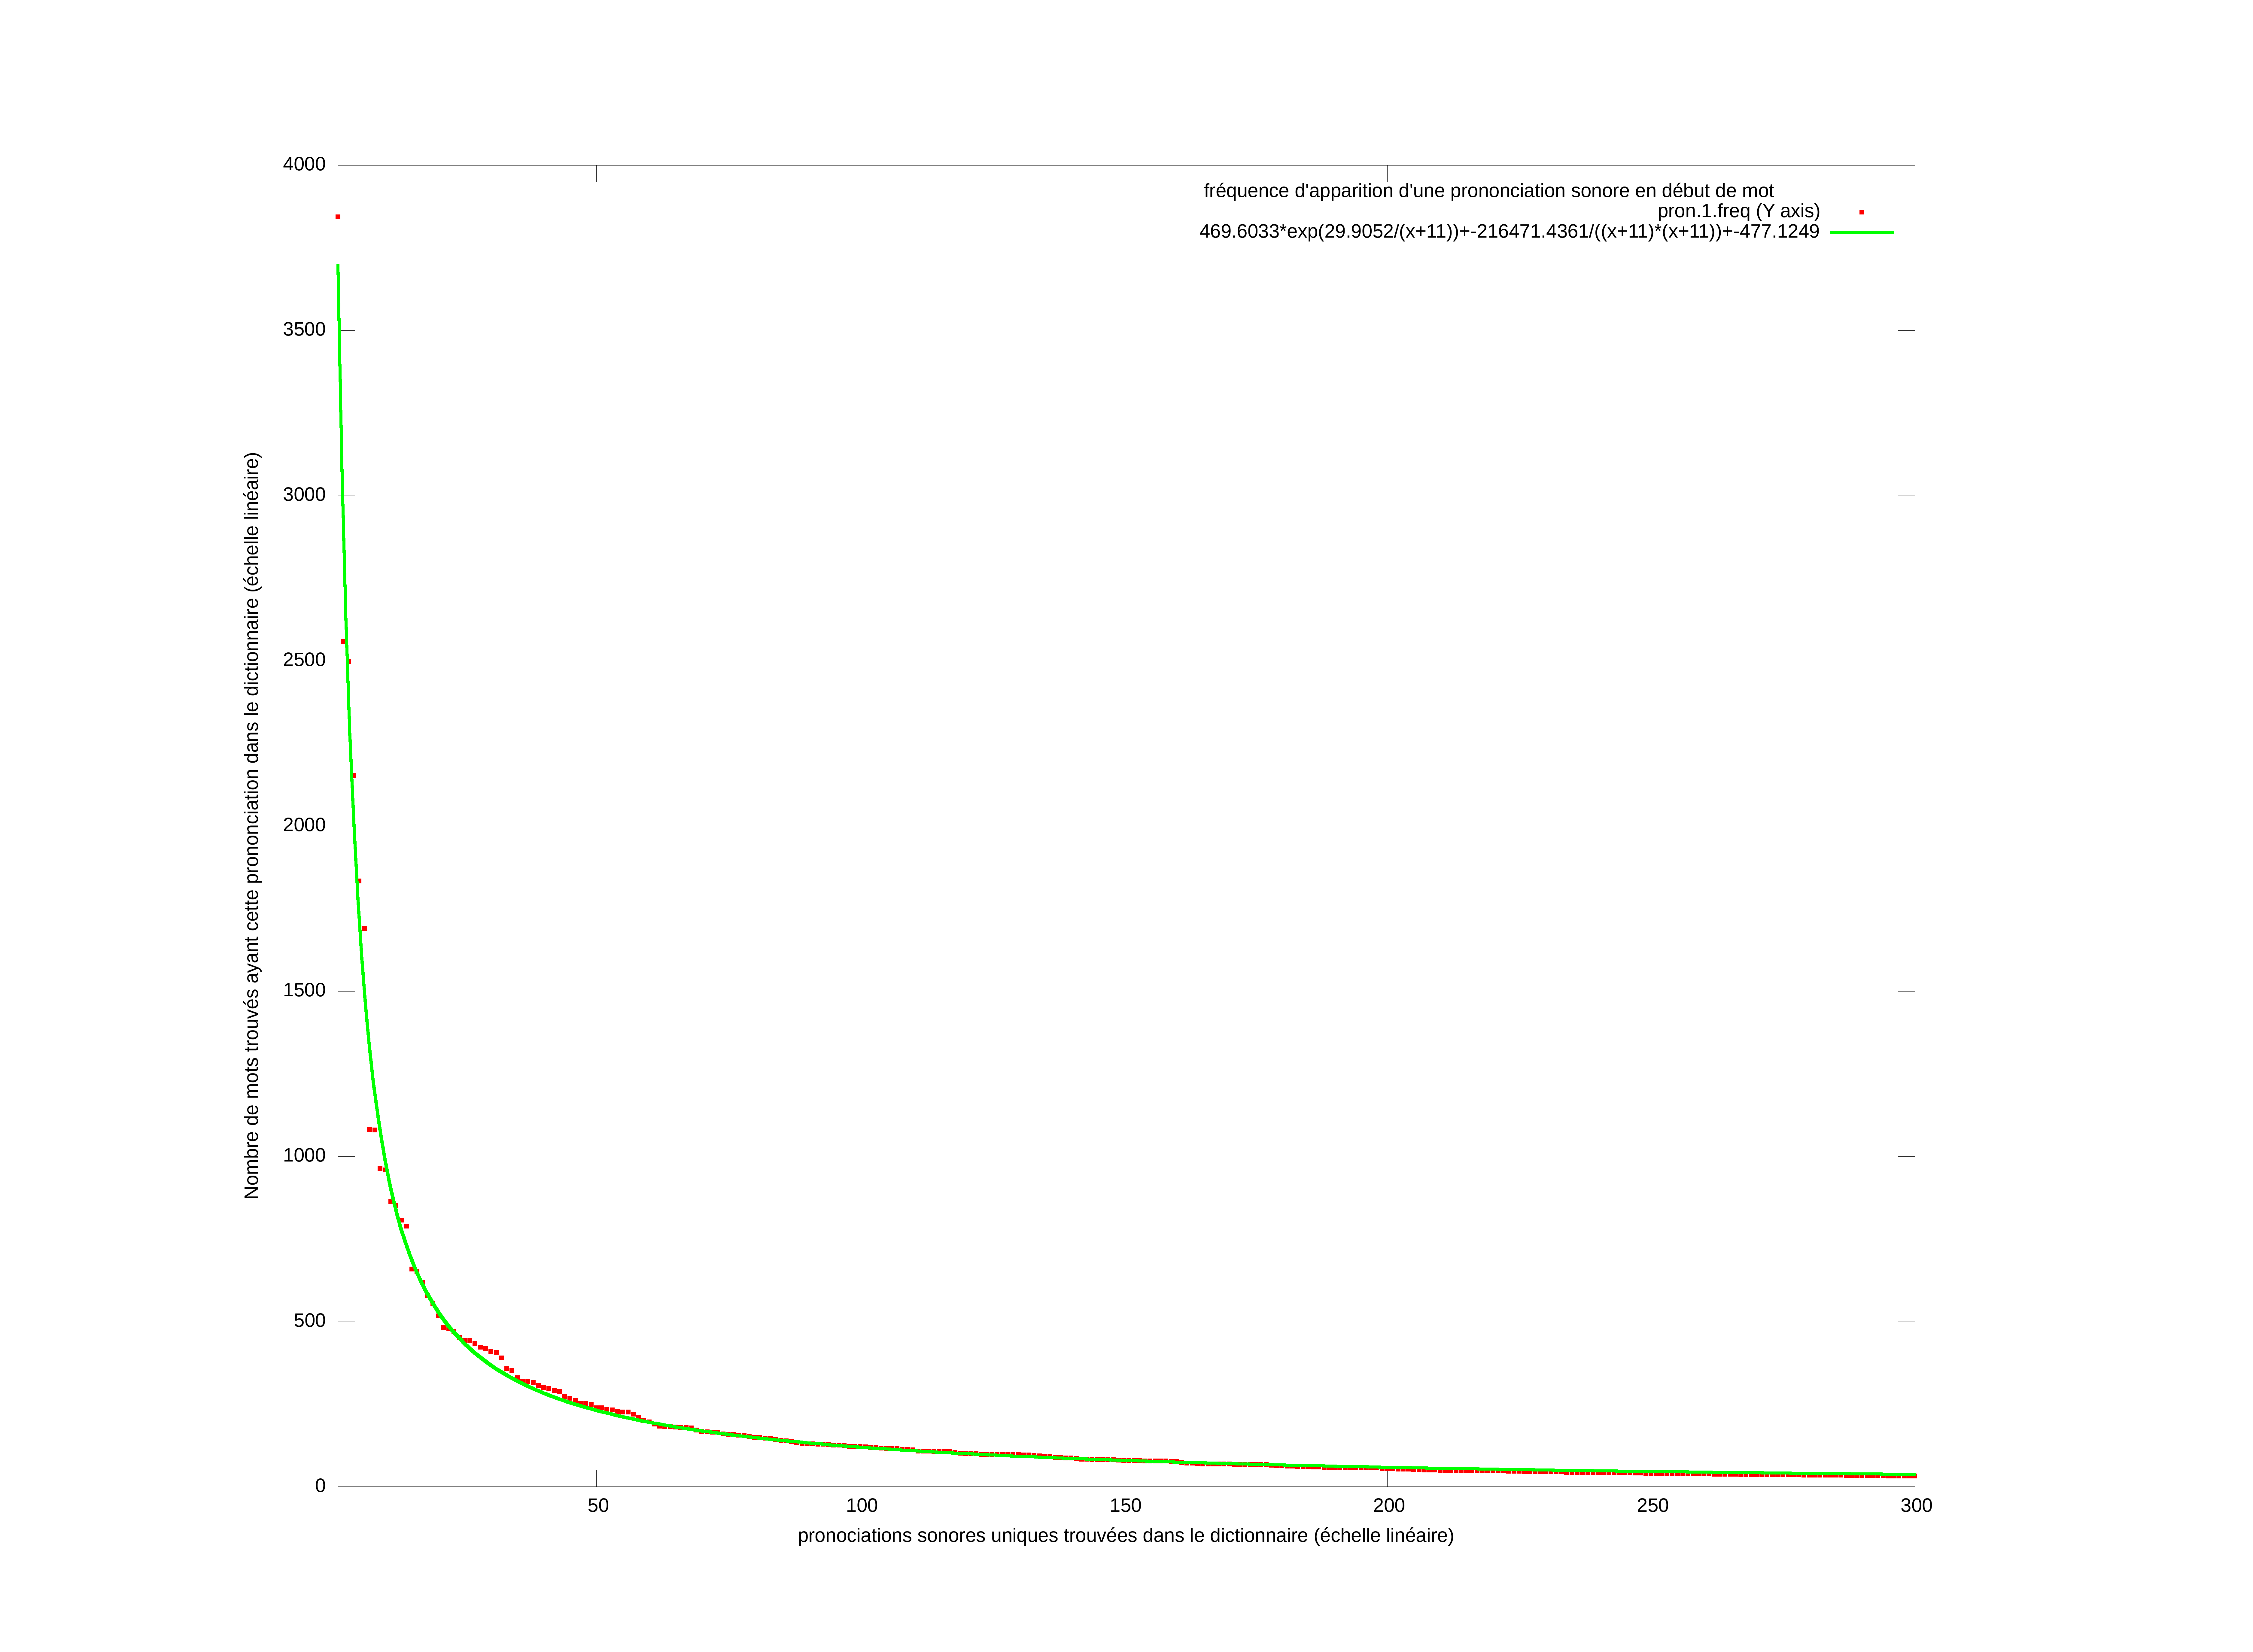
\includegraphics[width=\textwidth]{/home/olivier/Encfs/Privé/ENCRYPTED/Langages/developpement/poetry_analyze/french_with_prononc/gnuplot/pron.1.freq.png}
\underline{Recherche d'une formulation mathématique :}\\
\\
J'ai utilisé la commande "fit" de gnuplot avec différentes fonctions et en cherchant à diminuer la variance des résidus (variance of residuals (reduced chisquare), en anglais).\\
\\
Alors il est possible de déterminer une fonction approchante par interpolation linéaire : ce n'est donc qu'une approximation et n'a pas de valeur au sens rigoureux mathématiquement, même si j'aime bien sa forme :\\
\begin{center}
Soit $ \mathbf{x \in N, x > 0} $, et $ \mathbf{m \in N} $ tel que $ \mathbf{m = x + 11} $,\\
soit les variables $ \mathbf{\alpha, \beta, \gamma} $ et $ \mathbf{\phi \in R} $, alors\\
$ \mathbf{f(m) = \alpha * \exp(\beta/m) + \gamma / m^2 + \phi} $\\
est un fonction représentée en vert sur le graphe ci-dessus et approchant au mieux les données expérimentales partielles.\\
\end{center}
J'ai essayé la loi de distribution exponentielle-logarithme (EL) et la loi log-logistique, mais je n'ai pas réussi à approcher aussi bien les données expérimentales.\\
\\
La modélisation de la fonction est néanmoins un sujet à creuser : existe-t'il une courbe limite qui serait l'asymptote des rimes sonores de début et fin de mots ?\\
\\
On touche là, à la représentation des choses du monde par les mathématiques, les langues semblent bien s'approcher de lois mathématiques, assez simples par ailleurs, mais toujours aussi mystérieuses :-)\\
\\
\underline{Exemples}
\paragraph{5 mots dont le début de prononciation rime avec :\\}
\texttt{[\colorbox{blue}{\textipa{\~a\textyogh}}] : \colorbox{yellow}{\textbf{ange}}let,\colorbox{yellow}{\textbf{ange}}lot,\colorbox{yellow}{\textbf{ange}}vine,\colorbox{yellow}{\textbf{enge}}lure,\colorbox{yellow}{\textbf{ange}}}\\
\paragraph{24 mots dont le début de prononciation rime avec :\\}
\texttt{[\colorbox{blue}{k{\textipa{\textopeno}}k}] : \colorbox{yellow}{\textbf{coc}}cidie,\colorbox{yellow}{\textbf{coc}}cidiose,\colorbox{yellow}{\textbf{coc}}cinelle,\colorbox{yellow}{\textbf{coc}}cobacille,\colorbox{yellow}{\textbf{coc}}cygienne,\colorbox{yellow}{\textbf{coc}}hlée,\colorbox{yellow}{\textbf{cock}}ney,}\\
\texttt{\colorbox{yellow}{\textbf{cock}}pit,\colorbox{yellow}{\textbf{cock}}tail,\colorbox{yellow}{\textbf{coc}}tion,\colorbox{yellow}{\textbf{coque}}cigrue,\colorbox{yellow}{\textbf{coque}}let,\colorbox{yellow}{\textbf{coque}}lucheuse,\colorbox{yellow}{\textbf{coque}}luche,\colorbox{yellow}{\textbf{coq}}uemar,\colorbox{yellow}{\textbf{coque}}ron,}\\
\texttt{\colorbox{yellow}{\textbf{coque}}tier,\colorbox{yellow}{\textbf{coque}}tière,\colorbox{yellow}{\textbf{cox}}algie,\colorbox{yellow}{\textbf{cox}}algique,\colorbox{yellow}{\textbf{cox}}er,\colorbox{yellow}{\textbf{coke}},\colorbox{yellow}{\textbf{coque}},\colorbox{yellow}{\textbf{coq}}}\\
\subsection{Rimes sonores en fin de mots}
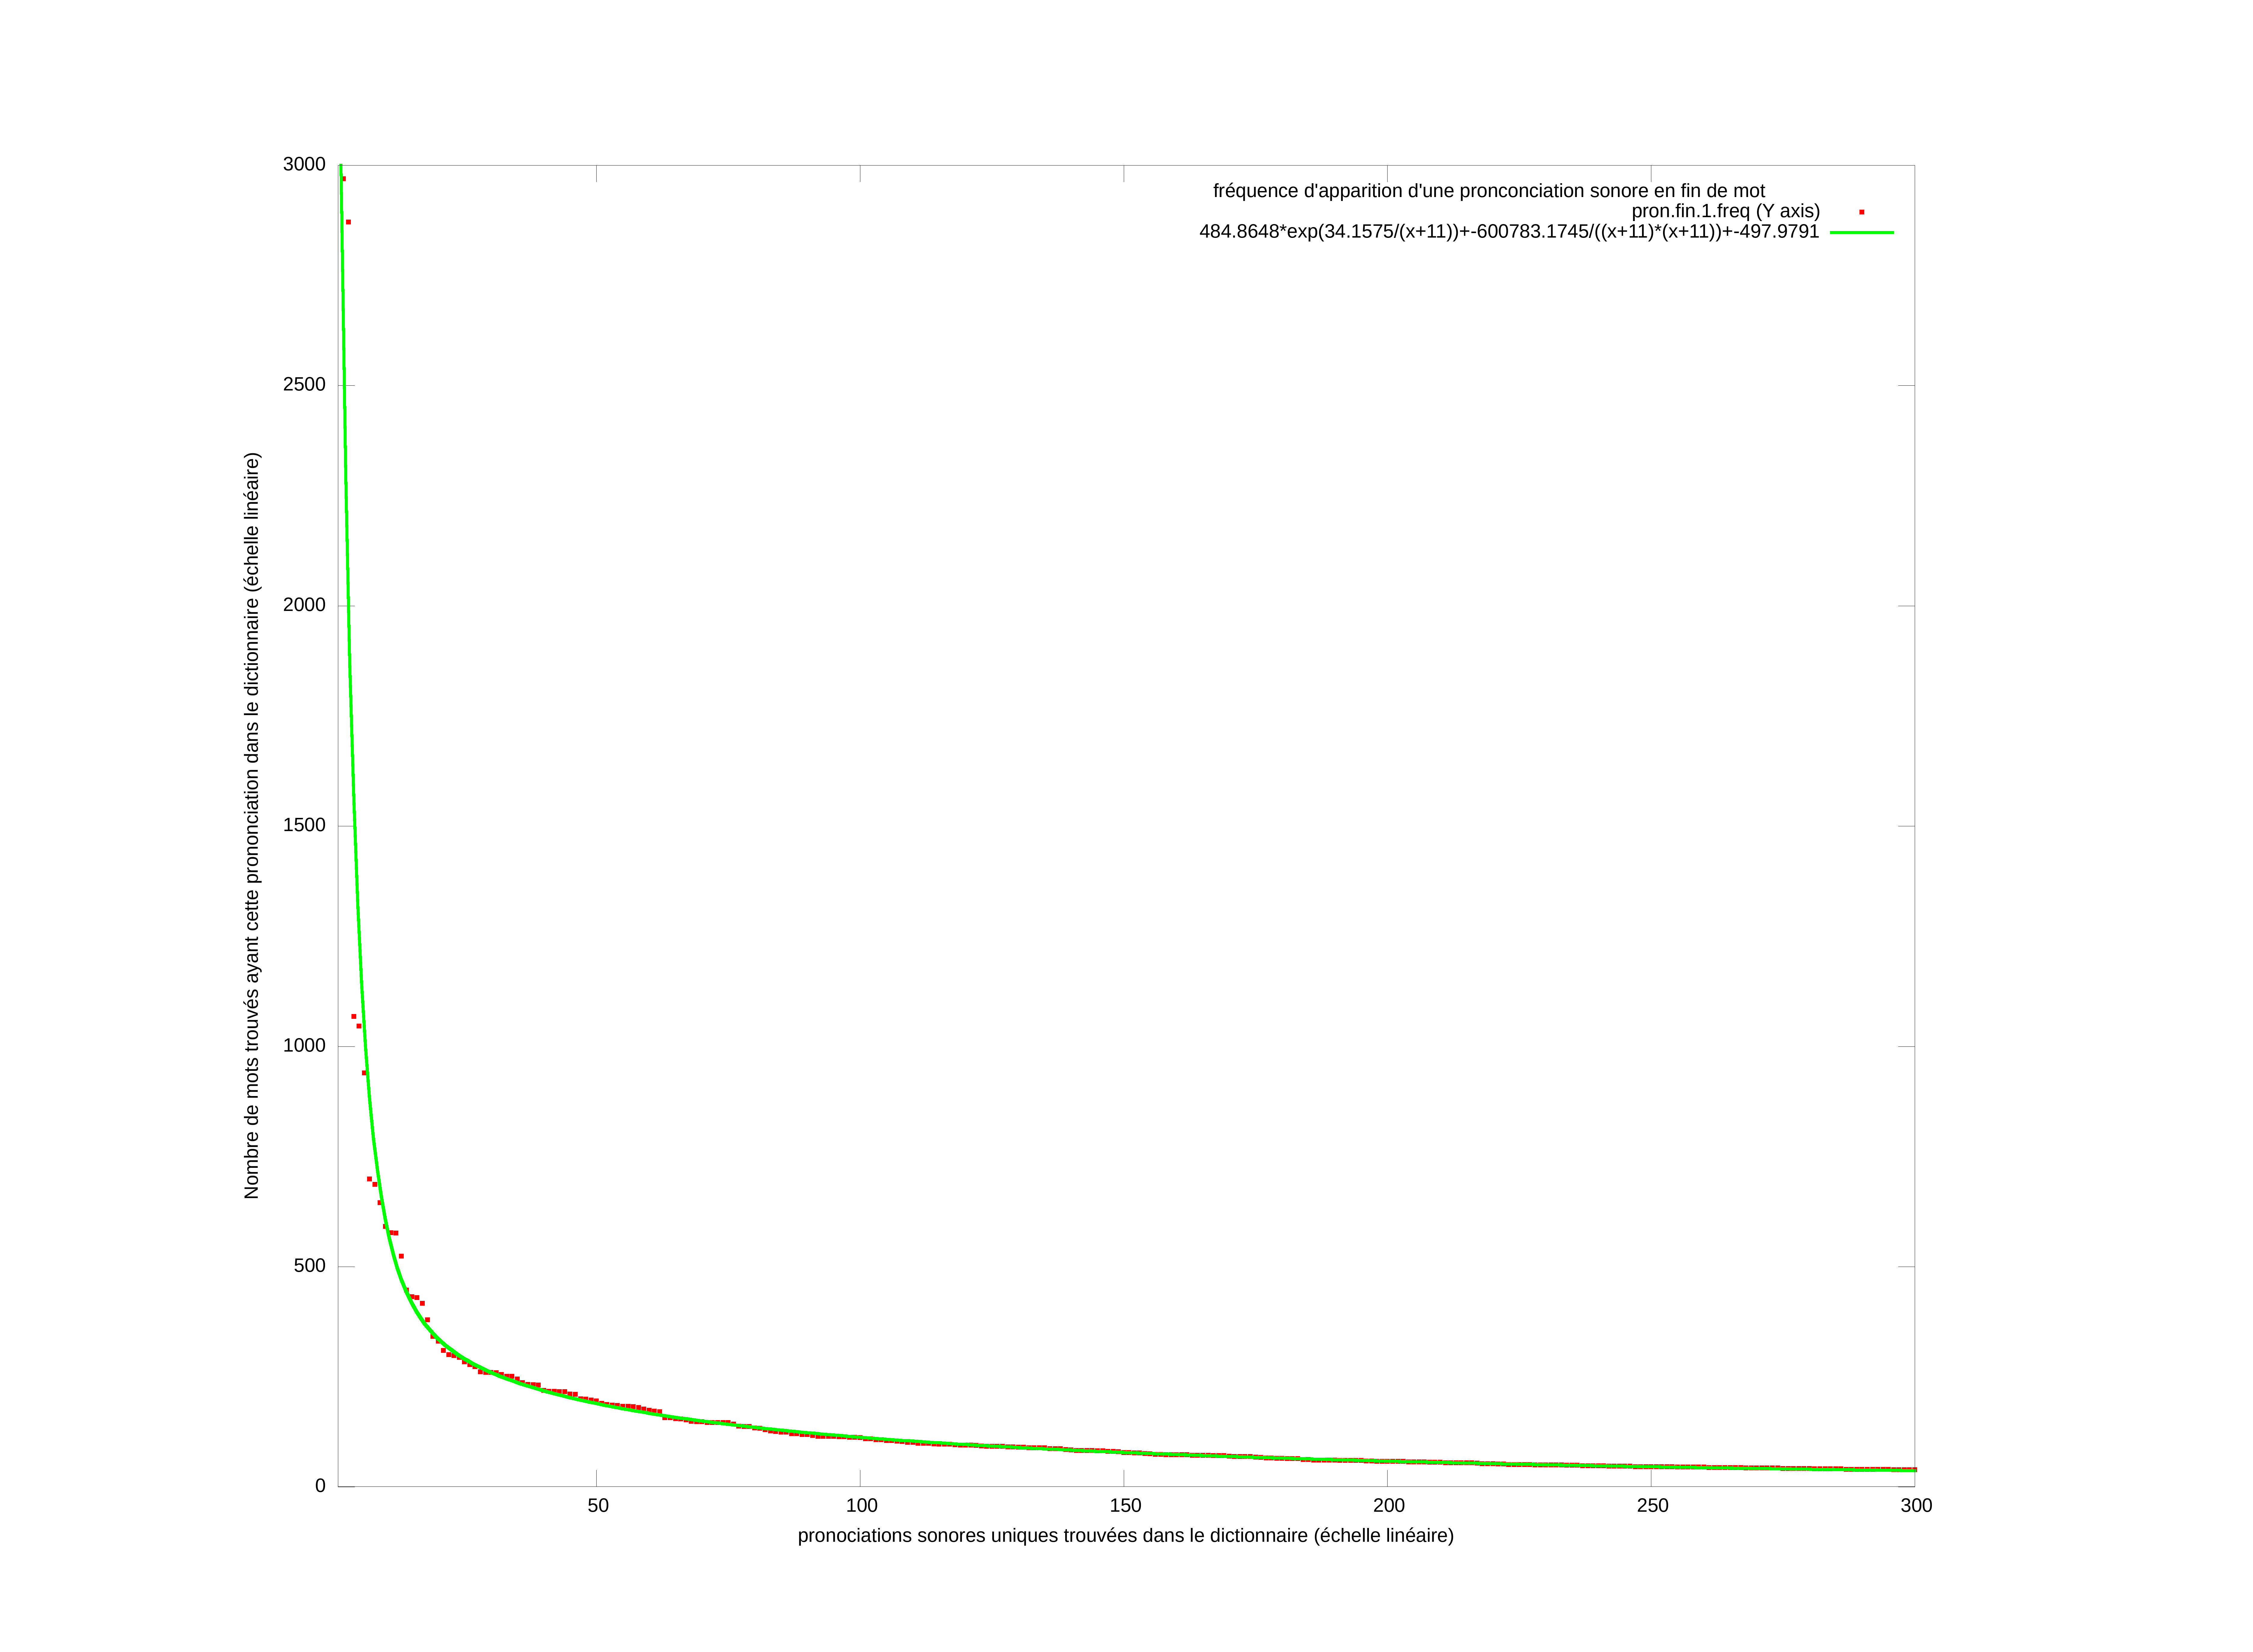
\includegraphics[width=\textwidth]{/home/olivier/Encfs/Privé/ENCRYPTED/Langages/developpement/poetry_analyze/french_with_prononc/gnuplot/pron.fin.1.freq.png}
\underline{Recherche d'une formulation mathématique :}\\
\\
J'ai également utilisé la commande "fit" de gnuplot.\\
\\
La forme de la fonction approchante par interpolation linéaire est la même que pour les rimes sonores en début de mots :\\
\begin{center}
Soit $ \mathbf{x \in N, x > 0} $, et $ \mathbf{m \in N} $ tel que $ \mathbf{m = x + 11} $,\\
soit les variables $ \mathbf{\alpha, \beta, \gamma} $ et $ \mathbf{\phi \in R} $, alors\\
$ \mathbf{f(m) = \alpha * \exp(\beta/m) + \gamma / m^2 + \phi} $\\
est un fonction représentée en vert sur le graphe ci-dessus et approchant au mieux les données expérimentales partielles.\\
\end{center}
\underline{Exemples}
\paragraph{2 mots dont la fin de prononciation rime avec :\\}
\texttt{[\colorbox{blue}{at{\textipa{\textinvscr}}}] : amphithé\colorbox{yellow}{\textbf{âtre}},bleu\colorbox{yellow}{\textbf{âtre}}}\\
\paragraph{6 mots dont la fin de prononciation rime avec :\\}
\texttt{[\colorbox{blue}{\textipa{\textyogh}o}] : bar\colorbox{yellow}{\textbf{jot}},bar\colorbox{yellow}{\textbf{jo}},ca\colorbox{yellow}{\textbf{geot}},do\colorbox{yellow}{\textbf{jo}},jo\colorbox{yellow}{\textbf{jo}},pa\colorbox{yellow}{\textbf{geot}}}\\
\newpage
\subsection{Expressions}
On prend 2964 expressions uniques de la langue française et on extrait tous les mots d'une certaine longueur, entre 3 lettres et 7 lettres en l'occurence.\\
\\Puis on dresse la liste des expressions qui contiennent chaque mot de 3 lettres (ou plus), une autre liste d'expressions qui contiennent chaque mot de 4 lettres ou plus, jusqu'à la liste d'expression qui contiennent chaque mot de 7 lettres ou plus.\\
\\Enfin, on comptabilise la somme des listes qui contiennent 2 expressions de mots de 3 lettres (ou plus), 3 expressions de mots de 3 lettres (ou plus), 4 expressions de mots de 3 lettres (ou plus), etc.\\
De même on comptabilise la somme des listes qui contiennent 2 expressions de mots de 4 lettres (ou plus), 3 expressions de mots de 4 lettres (ou plus), 4 expressions de mots de 4 lettres (ou plus), etc.\\
et ainsi de suite.\\
\\La fréquence de répartition des mots contenus dans les expressions, en fonction du nombre d'expressions peut être représentée sous forme de graphique.\\
\\Ce graphique de réparition des 345 mots uniques de 4 lettres trouvés dans 2964 expressions, ne montre pas de tendance asymptomatique des valeurs en Y :\\
\includegraphics[width=\textwidth]{/home/olivier/Encfs/Privé/ENCRYPTED/Langages/developpement/expressions_analyse/gnuplot/fréquence_de_répartition_des_345_mots_uniques_de_4_lettres_dans_2964_expressions_francaises_les_contenant.png}
\newpage
Par contre, lorsqu'on prend tous les mots uniques de 4 lettre ou plus, on arrive à la situation suivante :\\
\includegraphics[width=\textwidth]{/home/olivier/Encfs/Privé/ENCRYPTED/Langages/developpement/expressions_analyse/gnuplot/fréquence_de_répartition_des_2763_mots_uniques_de_4_lettres_ou_plus_contenus_dans_2964_expressions_francaises_les_contenant.png}
Si bien qu'on arrive à la même répartition asymptomatique : la forme de la fonction approchante par interpolation linéaire est la même que pour les rimes sonores :\\
\begin{center}
Soit $ \mathbf{x \in N, x > 0} $,\\
soit les variables $ \mathbf{\alpha, \beta, \gamma} $ et $ \mathbf{\phi \in R} $, alors\\
$ \mathbf{f(m) = \alpha * \exp(\beta/x) + \gamma / x^2 + \phi} $\\
est un fonction représentée en vert sur le graphe ci-dessus et approchant au mieux les données expérimentales partielles.\\
\end{center}
Il semble pourtant ne pas y avoir de rapports entre les deux, c'est toute  l'utilité de l'analyse de fréquence qui montre des rapports étroits entre la construction des expressions courantes de la langue française et les mots, ainsi que les rimes sonores et les mots.\\
\newpage
\section{Conclusions}
\subsection{Alors ces rimes ?}
Les règles de conjugaison impliquent forcément des rimes entre des préfixes commun, elles sont simples à détecter et à dénombrer dans la langue française.\\
Les rimes qui en sont issues ne sont pas forcément les plus intéressantes pour le poète.\\
Cependant les règles de conjugaison ne sont pas les seules à "forger" les rimes de la langue française (donner des exemple précis).\\
Le dénombrement des rimes a également jeté la lumière sur une dynamique mathématique des mots de la langue française, car des motifs géométriques sont apparus sur les représentations graphiques.
\subsection{Une langue vivante }
Par définition une langue vie par ceux qui la parlent, l'écrivent, et la lisent.\\
Et de nombreux mots disparaissent ou apparaissent chaque année dans les mises à jour des dictionnaires des éditeurs du marché.
\subsection{Métaphysique des rimes}
Nous pensons avoir un espace total de liberté d'écriture au sein de la langue française, alors que la structure même des mots répond à des contraintes mathématiques dont nous avons découvert une partie à l'occasion de cette analyse de rimes.\\
\\
L'utilisation de deux dictionnaires différents en taille et en typologie nous a permis de mettre en lumière que ces contraintes sont équivalentes si on rajoute des mots composés, comme "la convention internationale", ou des déclinaisons de conjugaison des verbes, comme "braver, braverai, braverais, bravera, aurait bravé, bravasse, etc."\\
\\
Ces contraintes mathématiques ne sont pas strictes, dans le sens où les rimes devraient obéir scrupuleusement à une équation, mais dans le sens asymptomatique, les valeurs mesurées de quantité de rimes tendant vers ce qu'on pourrait appeler des "attracteurs étranges", comme en théorie des fractales.\\
\\
Par conséquent, en plus de la dynamique d'ajout et de suppression de mots dans les dictionnaires en fonction du temps, citée précédemment, il y a également la découverte de nouveaux mots à formuler tout en respectant la limite asymptomatique du nombre de rimes en fonction de la taille des mots, sur l'ensemble des mots d'un dictionnaire.\\
\\
En particulier l'analyse des rimes glissantes (mais pas que), met à jour que la construction, le choix, d'un nouveau mot (ou de son abandon), est lié de façon subtilement mathématique à l'ensemble des autres mots déjà présents dans le dictionnaire de la langue française.
\subsection{Pour finir}
Un clin d'oeil à ces paroles encore de "Le Coq et la Pendule" où l'on voit bien que la poésie réserve bien des surprises : des mots inventés, comme "coqtambule" ou encore "ma poule aux heures d'or", sublimes inventions.. mais qui ne figurent pas dans un dictionnaire.
\newpage
\begin{appendix}
\section{Quelques réflexions sur la quantité de lignes de code nécessaires à ce travail de recherche}
Sans rentrer dans la technique, voici les différentes étapes qui ont émergées de mon étude :\\
La première étape fut de "transformer/nettoyer" le ou les dictionnaire(s) récupérés sur Internet, ainsi que le dictionnaire français embarqué dans le package Linux hunspell : \url{https://cran.r-project.org/web/packages/hunspell/vignettes/intro.html#hunspell_dictionaries}\\
\\
Ensuite vient l'étape d'indexation de ces dictionnaires en dictionnaires "partiels", c'est à dire ayant certaines propriétés, comme la taille des mots, etc.\\
\\
L'étape la plus importante est évidemment la recherche proprement dite des types de rimes dans la langue française.\\
\\
Vient enfin des calculs complémentaires (qui ne sont pas utiles pour l'analyse principale) sur la fréquence d'apparation de rimes ou de séquences  de rimes, et sur la "distance" métrique entre les mots.\\
Combien de lignes de code ont été requises pour arriver à ces fins ?\\
Là, il faut rentrer un tout petit peu dans les détails et connaître le Bash (sans rentrer dans le détail des scripts proprement dits) :\\
Un script de filtrage de mots du dictionnaire contenant précisement une taille précise de lettres :\\
\texttt{41 creation\_rev\_dic.sh}\\
il y a 4 types de dictionnaires générés :\\
- mots d'une taille précise faisant également partis du dictionnaire.\\
- mots d'une taille précise et n'ayant pas forcément de signification.\\
- mots "inversés" d'une taille précise faisant également partis du dictionnaire.\\
- mots "inversés" d'une taille précise et n'ayant pas forcément de signification.\\
et 2 dictionnaires contenant le symbole "\^" en début de mot pour faire une recherche efficace par la commande Unix \texttt{grep}\\
Le code source bash de traitement de recherche de rimes est le même en fin ou début de rimes, à ceci près que les dictionnaires utilisés pour le début de rimes sont les "inversés" des dictionnaires pour la fin de rimes (et qu'il faut "retourner" le texte satisfaisant à la recherche à l'aide de la commande "rev").\\
Par conséquent le nombre de lignes de code bash est strictement la même, mais pas le contenu, d'où les 2 scripts :\\
\texttt{54 rimes\_fin\_1.sh}\\
\texttt{54 rimes\_debut\_2.sh}\\
Même cas de figure pour les rimes de type 2 et 4 :\\
\texttt{49 rimes\_debut\_3.sh}\\
\texttt{49 rimes\_fin\_4.sh}\\
-> ces 2 scripts contiennent également quelques lignes de bash pour le calcul des fréquences d'apparition de séquences de rimes de taille différente.\\
Même cas de figure pour les rimes de type 5 et 6 :\\
\texttt{50 rimes\_fin\_5.sh}\\
\texttt{50 rimes\_debut\_6.sh}\\
Le cas des rimes glissantes est le plus ardu et contient logiquement plus de lignes de code :\
\texttt{116 rimes\_glissantes\_7.sh}\\
De plus, en extra (pas nécessaire pour la recherche de rimes), un script d'analyse de la distance de levhenstein :\\
\texttt{85 freq\_rimes.sh}\\
Ca fait donc un peu plus de trois cents lignes de code Bash pour rechercher les 7 types de rimes dans la langue française (lignes de commentaires inclues)\\
\newpage
En ce qui concerne les rimes sonores, c'est beaucoup plus simple :\\
\texttt{50 rimes\_sonore\_debut.sh}\\
\texttt{50 rimes\_sonore\_fin.sh}\\
\\Par défaut la recherche se limite à la première prononciation du mot et à la dernière, mais il est possible de demander une profondeur plus importante.\\
\\Enfin, en extra également, un script de génération de prononciations de mot, pour les mots dont la prononciation n'a pas été trouvée sur Internet (et il y en avait plusieurs milliers dans hunspell au moment de cette étude) :\\
\texttt{132 fonctions\_recherche\_phonetique.sh}\\
\texttt{133 recherche\_phonetique15.sh}\\
\\Sur cette recherche phonétique, le code shell est loin d'être aussi performant que dans un autre langage de programmation, mais ça fait l'affaire.\\
\section{Anecdote}
Pour l'anecdote, le code bash utilisé dans le cadre de cette étude est particulièrement optimisé, utilise des commandes Unix assez anciennes mais très efficaces, comme \texttt{sort, tr, sed, rev, cut, grep, paste, bc et awk}, ainsi que la commande \texttt{sponge} du package moreutils, assez peu utilisée mais particulièrement utile.\\
\\
Je suis fier de dire que ce sont mes plus intéressantes lignes de code shell depuis le début de ma carrière.\\
\\
Jamais je n'ai eu à utiliser ces commandes Unix de cette façon dans le cadre de mon activité professionnelle, ce qui est d'autant plus motivant pour l'esprit.\\
\\
Même s'il n'est pas question de performance de temps de calcul (ce qui nécessiterait beaucoup de développement et d'analyse complémentaire pour comparer avec d'autres langages de programmation), je pense que le ratio simplicité d'écriture/rapidité de calcul des traitements est particulièrement bonne.\\
\\
Car à part l'utilisation des boucles en Bash, qui sont peu performantes, j'ai utilisé des binaires dont le code source est lui très performant, ainsi que le parallélisme, qui a été utilisé aussi souvent que possible avec la soumission de jobs à l'ordonnanceur Linux en fond de tâche.\\
\section{Source des scripts et dictionnaires}
Le dictionnaire "dela" a été récupéré depuis :\\ \url{https://infolingu.univ-mlv.fr/DonneesLinguistiques/Dictionnaires/telechargement.html}.\\
\\Les ressources linguistiques disponibles par l'intermédiaire des boutons du site infolingu.univ-mlv.fr sont sous licence Lesser General Public License (LGPL) For Linguistic Resources.\\
Le dictionnaire hunspell a été récupéré depuis :\\ \url{https://github.com/elastic/hunspell/blob/master/dicts/fr/fr.dic}.\\
\\
Egalement l'ensemble des scripts shell de cette étude sont publiés avec la licence "GNU General Public License 3.0" sur Git :\\
\url{https://github.com/Ogaba/poetry_analyze}.\\
\section{Source des expressions}
Les 2 sources que j'ai récupérées sont :\\
\url{https://www.expressio.fr/documents/1000_expressions_preferees_des_francais_echantillon.pdf}\\
et\\
\url{http://docnum.univ-lorraine.fr/public/BUMED_MORT_2014_ETIENNE_ELODIE.pdf}\\
\\Note : je n'ai pas demandé l'autorisation des auteurs, mais j'espère qu'ils me pardonneront d'avoir seulement récupéré la liste des expressions françaises de leur document, dont personne ne peut revendiquer aujourd'hui en tout cas, la paternité..
\end{appendix}
\end{document}